%3.3 （LU分解代码不太显然）
%3.4 有大问题
%4.4 代码要大概
%7.6 概念要搞一搞代码重写

\pagenumbering{arabic}

\section{实验一}

\subsection*{1.1}
\addcontentsline{toc}{subsection}{1.1}
设方程 $f(x) = x^3 - 3x - 1 = 0$ 有 3 个实根：
\[
x_1^* = 1.8793, \quad x_2^* = -0.34727, \quad x_3^* = -1.53209
\]
采用下面六种不同计算格式，求 $f(x) = 0$ 的根 $x_1^*$ 或 $x_2^*$ 或 $x_3^*$ 的近似值，并考察相应格式的收敛性。

\begin{enumerate}
    \item $x_{k+1} = \frac{3x_k + 1}{x_k^2}, \quad k = 0, 1, 2, \ldots;$
    \item $x_{k+1} = \frac{x_k^3 - 1}{3}, \quad k = 0, 1, 2, \ldots;$
    \item $x_{k+1} = \sqrt[3]{3x_k + 1}, \quad k = 0, 1, 2, \ldots;$
    \item $x_{k+1} = \frac{1}{x_k^2 - 3}, \quad k = 0, 1, 2, \ldots;$
    \item $x_{k+1} = \sqrt{3 + \frac{1}{x_k}}, \quad k = 0, 1, 2, \ldots;$
    \item $x_{k+1} = x_k - \frac{1}{3} \left( \frac{x_k^3 - 3x_k - 1}{x_k^2 - 1} \right), \quad k = 0, 1, 2, \ldots.$
\end{enumerate}

我们直接代入每一种迭代函数挨个计算即可。

\begin{lstlisting}[language=matlab]
clc; clear;
% 随便设的，第二个设为1是因为它在2是发散的。
x0_list = [2, 1, 2, 2, 2, 2];
% 最大迭代次数
N = 20;
iters = {
    @(x) (3*x + 1)./x.^2;                           
    @(x) (x.^3 - 1)/3;                              
    @(x) nthroot(3*x + 1, 3);                       
    @(x) 1./(x.^2 - 3);                             
    @(x) sqrt(3 + 1./x);                            
    @(x) x - (1/3)*( (x.^3 - 3*x - 1)./(x.^2 - 1) );
};

titles = {
    'x_{k+1} = (3x_k + 1)/x_k^2';
    'x_{k+1} = (x_k^3 - 1)/3';
    'x_{k+1} = \root{3}(3x_k + 1)';
    'x_{k+1} = 1 / (x_k^2 - 3)';
    'x_{k+1} = \surd(3 + 1/x_k)';
    'x_{k+1} = x_k - (1/3)*(f(x_k)/(x_k^2 - 1))';
};

% 迭代并绘图
for i = 1:6
    figure;  % 新建图窗
    x = zeros(1, N+1);
    x(1) = x0_list(i);
    for k = 1:N
        try
            x(k+1) = iters{i}(x(k));
        catch
            x(k+1) = NaN;
        end
    end
    
    plot(0:N, x, '-o', 'LineWidth', 1.5);
    hold on;
    yline(x_star, '--r', '$x^*$', 'Interpreter', 'latex');
    title(['格式 ' num2str(i) ': ' titles{i}], 'Interpreter', 'latex');
    xlabel('迭代次数 $k$', 'Interpreter', 'latex');
    ylabel('$x_k$', 'Interpreter', 'latex');
    legend({'$x_k$', '$x^*$'}, 'Interpreter', 'latex', 'Location', 'best');
    grid on;
end
\end{lstlisting}

\begin{figure}[htbp]
\centering
    \begin{minipage}{0.49\linewidth}
    \centering
    
\includegraphics[width=1\linewidth]{figure/1-1-1.png}
    \label{1-1-1}
    \label{chutian1}
    \end{minipage}
    \begin{minipage}{0.49\linewidth}
    \centering
    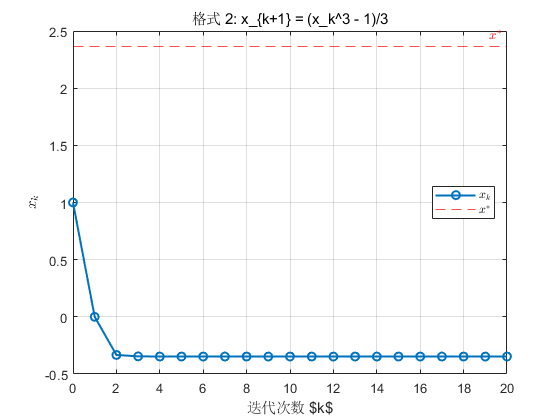
\includegraphics[width=1\linewidth]{figure/1-1-2.png}
    \label{1-1-2}
    \end{minipage}

    \begin{minipage}{0.49\linewidth}
    \centering
    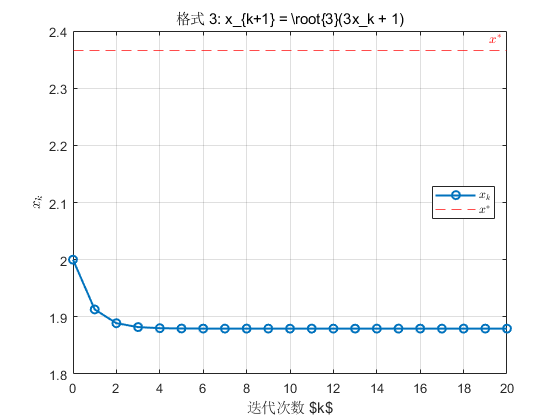
\includegraphics[width=1\linewidth]{figure/1-1-3.png}
    \label{1-1-3}
    \end{minipage}
    \begin{minipage}{0.49\linewidth}
    \centering
    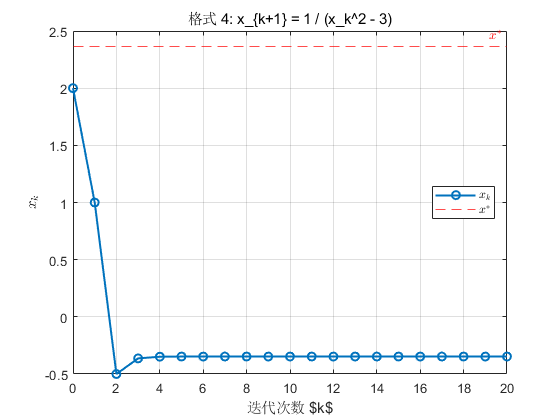
\includegraphics[width=1\linewidth]{figure/1-1-4.png}
    \label{1-1-4}
    \end{minipage}

    \begin{minipage}{0.49\linewidth}
    \centering
    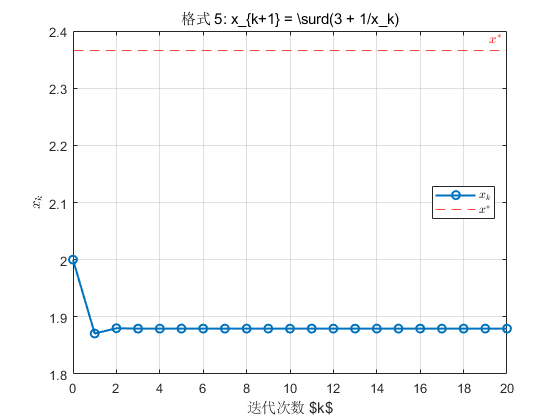
\includegraphics[width=1\linewidth]{figure/1-1-5.png}
    \label{1-1-5}
    \end{minipage}
    \begin{minipage}{0.49\linewidth}
    \centering
    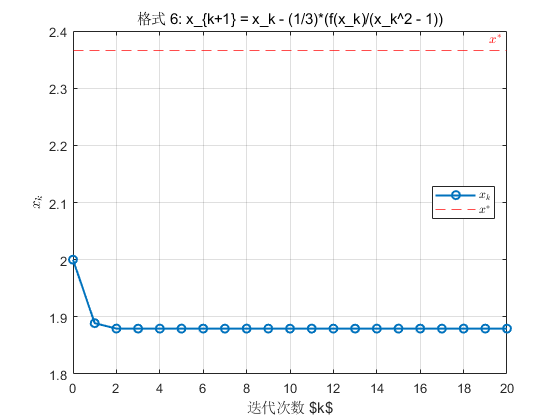
\includegraphics[width=1\linewidth]{figure/1-1-6.png}
    \label{1-1-6}
    \end{minipage}
\end{figure}

\subsection*{1.2}
\addcontentsline{toc}{subsection}{1.2}
一个 10 次多项式(非线性方程组求解)
$$
P(x) = x^{10} + a_1 x^9 + a_2 x^8 + \cdots + a_9 x + a_{10}
$$
系数为：$1, -55, 1320, -18150, 157773, -902055, 3416930, -8409500, 12753576, -10628640, 6328800$

\begin{enumerate}
    \item 用多项式的求根指令 roots 求出方程 \(P(x) = 0\) 的 10 个根；
    \item 试设计一个算法，求出方程 \(P(x) = 0\) 的 10 个根的近似值，并与(1)的结果进行比较；
    \item 将方程 \(P(x) = 0\) 左边多项式 \(P(x)\) 中的 9 次项的系数 \(-55\) 改为 \(-56\)，得到一个新的 10 次方程，求解新的方程，观察根的变化是否很显著，说明了什么？
\end{enumerate}

\begin{enumerate}
    \item 直接调用函数即可；
    \item 我们使用牛顿迭代法随意求出一个根$x_1$，之后使用多项式除法对原多项式除以 $(x-x_1)$，之后再次使用牛顿迭代法，不断重复此过程即可找到十个根；
    \item 更改参数直接调用函数即可。
\end{enumerate}



\begin{lstlisting}[language=matlab]
clc; clear;
coeffs = [1, -55, 1320, -18150, 157773, -902055, ...
           3416930, -8409500, 12753576, -10628640, 6328800];

% 求根
roots1 = roots(coeffs);

% 输出根
disp('原方程 P(x) = 0 的十个根：');
disp(roots1);


max_iter = 100;
tol = 1e-10;
poly = coeffs;
found_roots = [];

for k = 1:10
    x = 1 + 0.5 * exp(2i * pi * k / 11);  % 初始猜测
    % Newton 迭代
    for iter = 1:max_iter
        fx = polyval(poly, x);
        dfx = polyval(polyder(poly), x);  % 导数
        if dfx == 0
            break;
        end
        x_new = x - fx / dfx;
        if abs(x_new - x) < tol
            break;
        end
        x = x_new;
    end
    % 保存当前根
    found_roots(end+1) = x;
    % 用 (x - r) 除掉当前根，更新多项式
    [poly, ~] = deconv(poly, [1, -x]);  % 多项式除法
end

% 显示结果
disp('牛顿法逐步求得的近似根：');
disp(found_roots.');
% 比较误差
fprintf('最大与 roots 的差异: %.2e\n', max(abs(sort(roots1) - sort(found_roots.'))));
coeffs(2) = -56;
% 求新方程根
roots3 = roots(coeffs);
% 输出
disp('修改后的新方程 P*(x) = 0 的十个根：');
disp(roots3);
% 对比变化
fprintf('最大根变化量: %.3e\n', max(abs(sort(roots1) - sort(roots3))));
\end{lstlisting}

\begin{lstlisting}[language=matlab]
原方程 P(x) = 0 的十个根：
           10.6050883092581 +      1.01269519413022i
           10.6050883092581 -      1.01269519413022i
           8.58498741250269 +      2.78982117824004i
           8.58498741250269 -      2.78982117824004i
           5.49999999999931 +      3.50582949324341i
           5.49999999999931 -      3.50582949324341i
           2.41501258750811 +      2.78982117823975i
           2.41501258750811 -      2.78982117823975i
          0.394911690731821 +      1.01269519415343i
          0.394911690731821 -      1.01269519415343i

牛顿法逐步求得的近似根：
          0.394911690731822 +      1.01269519415343i
           8.58498741250564 -      2.78982117825771i
          0.394911690716699 -      1.01269519411747i
           2.41501258742504 -       2.7898211782494i
           5.50000000005835 +      3.50582949334393i
            10.605088309282 +      1.01269519408036i
           8.58498741260846 +      2.78982117822905i
           5.49999999996888 -      3.50582949331848i
           2.41501258747357 +      2.78982117829388i
           10.6050883092296 -      1.01269519415757i

最大与 roots 的差异: 1.17e-10
修改后的新方程 P*(x) = 0 的十个根：
           21.7335121408967 +                     0i
           7.35013402487902 +      7.79728509446718i
           7.35013402487902 -      7.79728509446718i
            4.3588618522737 +      3.32854671238129i
            4.3588618522737 -      3.32854671238129i
           5.18307297176246 +                     0i
           2.43780006851531 +      2.79739872415425i
           2.43780006851531 -      2.79739872415425i
          0.394911498002446 +      1.01269497774644i
          0.394911498002446 -      1.01269497774644i

最大根变化量: 1.117e+01
\end{lstlisting}

\subsection*{1.3}
\addcontentsline{toc}{subsection}{1.3}
找出方程 $x^3 + 2x - 5 = 0$ 的有根区间，再分别用二分法、不动点迭代法(取迭代函数 $\varphi_1(x) = \sqrt[3]{5-2x}$)、Newton 迭代法、弦截法、Steffensen 迭代法分别求方程 $x^3 + 2x - 5 = 0$ 的根。要求 $|x_{k+1} - x_k| < 10^{-6}$。（非线性方程组求解）

注意到函数在实数域是增函数，在$1$处为负，在$2$处为正，故$(0,2)$是一个有根区间。

关于Steffensen 迭代法上课没教，代入公式$x_{k+1}=x_k-\frac{(f(x_k)-x_k)^2}{f(f(x_k))-2f(x_k)+x_k}$，直接代码实现即可。

\begin{lstlisting}[language=matlab]
f = @(x) x.^3 + 2*x - 5;
% 搜索有根区间
x_vals = linspace(0, 2, 1000);
y_vals = f(x_vals);
plot(x_vals, y_vals); grid on;
xlabel('x'); ylabel('f(x)');
title('f(x) = x^3 + 2x - 5');

df = @(x) 3*x.^2 + 2;                   % Newton法用
phi1 = @(x) (5 - 2*x).^(1/3);           % 不动点法
eps = 1e-6;

a = 1; b = 2;
fa = f(a); fb = f(b);
if fa * fb > 0
    error('区间内无根');
end

while (b - a)/2 > eps
    c = (a + b)/2;
    fc = f(c);
    if fc == 0
        break;
    elseif fa * fc < 0
        b = c;
        fb = fc;
    else
        a = c;
        fa = fc;
    end
end
root_bisection = (a + b)/2;
fprintf('二分法根: %.10f\n', root_bisection);


x0 = 1.5;
x1 = phi1(x0);
while abs(x1 - x0) > eps
    x0 = x1;
    x1 = phi1(x0);
end
root_fixed = x1;
fprintf('不动点迭代法根: %.10f\n', root_fixed);

x0 = 1.5;
x1 = x0 - f(x0)/df(x0);
while abs(x1 - x0) > eps
    x0 = x1;
    x1 = x0 - f(x0)/df(x0);
end
root_newton = x1;
fprintf('Newton法根: %.10f\n', root_newton);


x0 = 1; x1 = 2;
while abs(x1 - x0) > eps
    x2 = x1 - f(x1)*(x1 - x0)/(f(x1) - f(x0));
    x0 = x1;
    x1 = x2;
end
root_secant = x1;
fprintf('弦截法根: %.10f\n', root_secant);


x0 = 1.5;
while true
    y = phi1(x0);
    z = phi1(y);
    denom = z - 2*y + x0;
    if denom == 0
        break;
    end
    x1 = x0 - ((y - x0)^2) / denom;
    if abs(x1 - x0) < eps
        break;
    end
    x0 = x1;
end
root_steff = x1;
fprintf('Steffensen法根: %.10f\n', root_steff);
\end{lstlisting}

\begin{lstlisting}[language=matlab]
二分法根: 1.3282690048
不动点迭代法根: 1.3282690715
Newton法根: 1.3282688557
弦截法根: 1.3282688557
Steffensen法根: 1.3282688557
\end{lstlisting}


\subsection*{1.4}
\addcontentsline{toc}{subsection}{1.4}
用牛顿切线法的局部收敛性判别方程 $e^x \sin x = 4$ 的近似根时，分别由不同的初始值 $x_0$：（1）$x_0 = -1$；（2）$x_0 = 0$；（3）$x_0 = 1$；（4）$x_0 = 2$；（5）$x_0 = 5.5$；（6）$x_0 = 8$，考察产生的迭代序列是否收敛？再用抛物线法求方程 $f(x) = e^{2x} - 3x^2 = 0$ 的一个实根的近似值 $x_k$，使精确到 $\varepsilon = 10^{-4}$。

抛物线法，即：以$x_{k-2},x_{k-1},x_k$三点的二次插值多项式的零点作为$x_{k+1}$，进行迭代。

\begin{lstlisting}[language=matlab]
clc; clear;
f = @(x) exp(x).*sin(x) - 4;
df = @(x) exp(x).*(sin(x) + cos(x));
eps = 1e-10;
max_iter = 100;
x0_list = [-1, 0, 1, 2, 5.5, 8];

fprintf('Newton 法收敛性分析:\n');
for i = 1:length(x0_list)
    x0 = x0_list(i);
    fprintf('\n初值 x0 = %.2f:\n', x0);
    diverged = false;
    
    for k = 1:max_iter
        fx = f(x0);
        dfx = df(x0);
        if dfx == 0
            fprintf('  第 %d 步导数为 0，停止。\n', k);
            diverged = true;
            break;
        end
        x1 = x0 - fx / dfx;
        if isnan(x1) || isinf(x1)
            fprintf('  第 %d 步发散 (NaN/Inf)。\n', k);
            diverged = true;
            break;
        end
        if abs(x1 - x0) < eps
            fprintf('  收敛到 x = %.6f (用 %d 步)\n', x1, k);
            break;
        end
        x0 = x1;
    end
    if ~diverged && k >= max_iter
        fprintf('  超过最大迭代步数，未收敛。\n');
    end
end

f = @(x) exp(2*x) - 3*x.^2;
eps = 1e-4;

% 初始三个点
x0 = 0; x1 = -0.5; x2 = -1;

for k = 1:100
    % 对应函数值
    y0 = f(x0); y1 = f(x1); y2 = f(x2);
    
    % 抛物线插值系数 a, b, c for P(x) = a(x-x2)^2 + b(x-x2) + c
    % c即为 f(x2)
    % 牛顿差商法
    h0 = x0 - x2; h1 = x1 - x2;
    f0 = y0; f1 = y1; f2 = y2;
    
    d0 = (f0 - f2) / h0;
    d1 = (f1 - f2) / h1;
    a = (d0 - d1) / (h0 - h1);
    b = a*h1 + d1;
    c = f2;

    delta = -2*c / (b + sign(b)*sqrt(b^2 - 4*a*c));  % 防止除零
    x_new = x2 + delta;

    if abs(x_new - x2) < eps
        fprintf('\n抛物线法求得实根 x = %.6f (迭代步 %d)\n', x_new, k);
        break;
    end

    % 更新点 (x0, x1, x2)
    x0 = x1;
    x1 = x2;
    x2 = x_new;
end
\end{lstlisting}

\begin{lstlisting}[language=matlab]
Newton 法收敛性分析:

初值 x0 = -1.00:
  第 3 步导数为 0，停止。

初值 x0 = 0.00:
  收敛到 x = 2.925321 (用 8 步)

初值 x0 = 1.00:
  收敛到 x = 1.400812 (用 5 步)

初值 x0 = 2.00:
  收敛到 x = 1.400812 (用 5 步)

初值 x0 = 5.50:
  收敛到 x = 235.619449 (用 7 步)

初值 x0 = 8.00:
  收敛到 x = 6.290600 (用 7 步)

抛物线法求得实根 x = -0.390646 (迭代步 10)
\end{lstlisting}

验证结果发现$x = 235.619449$函数值非常大，这是由于指数爆炸导致的，注意到$x=235.61945$的函数值与其差约为$1e100$，故可以认为这的确是一个近似零点。

\section{实验二}
\subsection*{2.1}
\addcontentsline{toc}{subsection}{2.1}
用 Taylor 级数的第 i 项多项式 $p_i(x)$ ($i = 1, 2, \cdots, 30$)，分别在区间 $[0, \frac{\pi}{2}]$ 和 $[0, \pi]$ 上逼近正弦函数 $f(x) = \cos x, \, x \in [0, \pi]$，并用计算机绘出上面 31 个函数的图形。

Taylor 展开式回顾（以 $x=0$ 展开）：

$$
\cos x = \sum_{n=0}^{\infty} \frac{(-1)^n x^{2n}}{(2n)!}
$$

第 $i$ 项多项式定义为：

$$
p_i(x) = \sum_{n=0}^{\lfloor i/2 \rfloor} \frac{(-1)^n x^{2n}}{(2n)!}
$$

\begin{lstlisting}[language=matlab]
x = linspace(0, pi, 500);
fx = cos(x);

figure;

% 我们想画的是 0-9, 10-19, 20-30 这三组（最后一组包含11项）
k_list = {0:9, 10:19, 20:30};

for fig_id = 1:3
    figure;
    plot(fig_id);
    plot(x, fx, 'k', 'LineWidth', 2); hold on;

    k_range = k_list{fig_id};
    for i = k_range
        p = zeros(size(x));
        for n = 0:floor(i/2)
            p = p + ((-1)^n * x.^(2*n)) / factorial(2*n);
        end
        plot(x, p);
    end

    title(sprintf('Taylor 多项式逼近 cos(x)（p_{%d} 到 p_{%d}）', ...
        k_range(1), k_range(end)));
    xlabel('x'); ylabel('y');
    legend_entries = arrayfun(@(k) sprintf('p_{%d}(x)', k), k_range, 'UniformOutput', false);
    legend(['cos(x)', legend_entries], 'Location', 'best');
    grid on;
end

\end{lstlisting}

\begin{figure}[htbp]
\centering
    \begin{minipage}{0.49\linewidth}
    \centering
    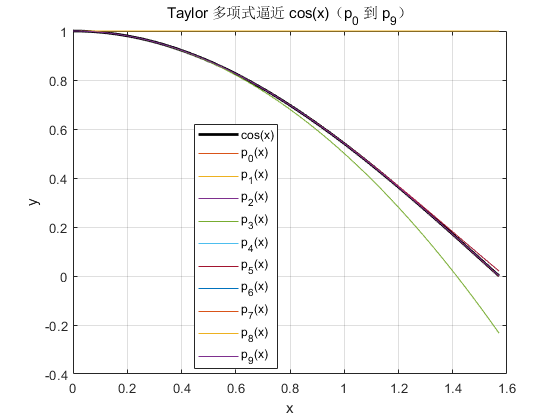
\includegraphics[width=1\linewidth]{figure/2-1-1.png}
    \label{2-1-1}
    \label{chutian1}
    \end{minipage}
    \begin{minipage}{0.49\linewidth}
    \centering
    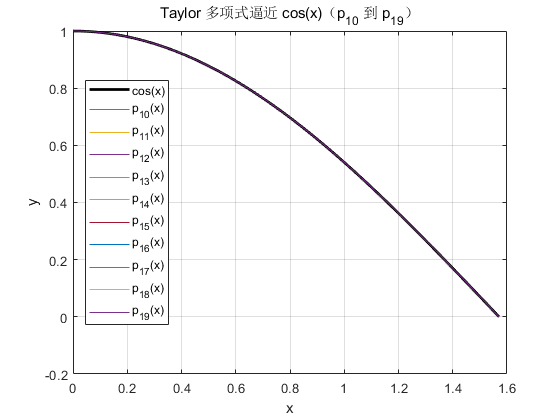
\includegraphics[width=1\linewidth]{figure/2-1-2.png}
    \label{2-1-2}
    \end{minipage}

    \begin{minipage}{0.49\linewidth}
    \centering
    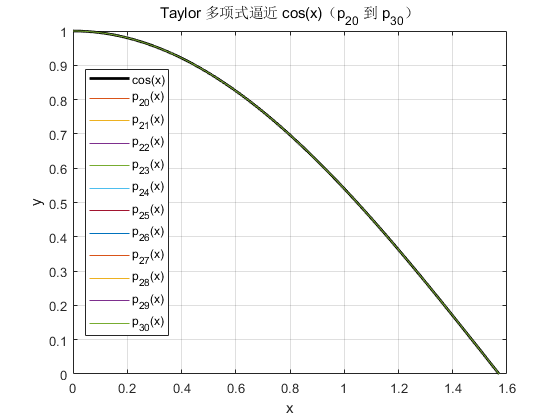
\includegraphics[width=1\linewidth]{figure/2-1-3.png}
    \label{2-1-3}
    \end{minipage}
    \begin{minipage}{0.49\linewidth}
    \centering
    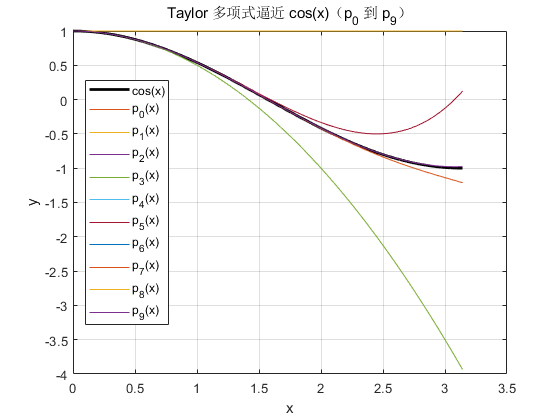
\includegraphics[width=1\linewidth]{figure/2-1-4.png}
    \label{2-1-4}
    \end{minipage}

    \begin{minipage}{0.49\linewidth}
    \centering
    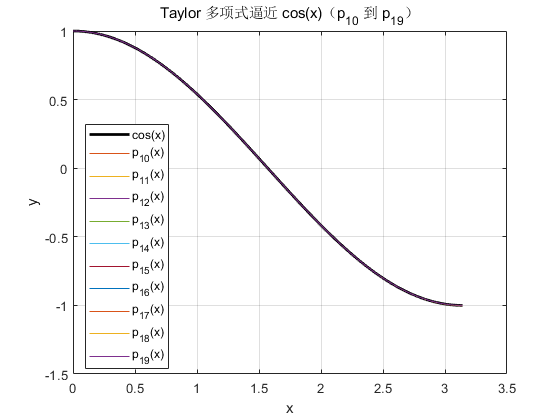
\includegraphics[width=1\linewidth]{figure/2-1-5.png}
    \label{2-1-5}
    \end{minipage}
    \begin{minipage}{0.49\linewidth}
    \centering
    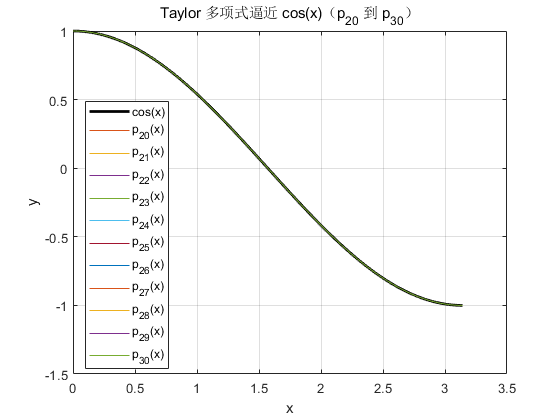
\includegraphics[width=1\linewidth]{figure/2-1-6.png}
    \label{2-1-6}
    \end{minipage}
\end{figure}


\subsection*{2.2}
\addcontentsline{toc}{subsection}{2.2}
\begin{enumerate}
    \item 已知函数 $f(x) = \cos(\pi x)$ 在节点 $x = 0, \, 0.25, \, 0.5, \, 0.75, \, 1.0$ 处的值，求满足边界条件 $f'(0) = 0$ 和 $f'(1.0) = 0$ 的三次样条插值函数 $S(x)$；
    \item 计算 $\int_0^1 S(x) dx$，并计算 $\int_0^1 f(x) dx - \int_0^1 S(x) dx$；
    \item 用 $S'(0.5)$ 和 $S''(0.5)$ 分别近似 $f'(0.5)$ 和 $f''(0.5)$。
\end{enumerate}

\begin{lstlisting}[language=matlab]
x = 0:0.25:1;
y = cos(pi*x);
fp0 = 0;             % f'(0) = 0
fp1 = 0;             % f'(1) = 0
% clamped spline 固定边界
pp = spline(x, [fp0 y fp1]);  % 在y两端添加导数作为边界条件

% 画出插值函数
xx = linspace(0, 1, 100);
yy = ppval(pp, xx);

figure;
fplot(@(x) cos(pi*x), [0 1], 'k--', 'DisplayName', 'f(x)=cos(\pi x)');
hold on;
plot(xx, yy, 'b-', 'DisplayName', 'S(x)');
plot(x, y, 'ro', 'DisplayName', 'Interpolation nodes');
legend;
title('三次样条插值函数 S(x)');
xlabel('x'); ylabel('y');
grid on;

fprintf('\n三次样条段函数系数 (每行代表一段: [a b c d], 表示 a*x^3 + b*x^2 + c*x + d)：\n');
disp(pp.coefs);

S_int = integral(@(x) ppval(pp, x), 0, 1);  % ∫₀¹ S(x) dx
f_int = integral(@(x) cos(pi*x), 0, 1);    % ∫₀¹ f(x) dx
error = f_int - S_int;

fprintf('∫₀¹ S(x) dx = %.8f\n', S_int);
fprintf('∫₀¹ f(x) dx - ∫₀¹ S(x) dx = %.8e\n', error);

pp_der1 = fnder(pp, 1);  % 一阶导
pp_der2 = fnder(pp, 2);  % 二阶导

S1 = ppval(pp_der1, 0.5);
S2 = ppval(pp_der2, 0.5);

f1 = -pi * sin(pi*0.5);
f2 = -pi^2 * cos(pi*0.5);

fprintf('S''(0.5) ≈ %.8f,   f''(0.5) ≈ %.8f,   误差 = %.2e\n', S1, f1, abs(S1 - f1));
fprintf('S''''(0.5) ≈ %.8f,  f''''(0.5) ≈ %.8f,  误差 = %.2e\n', S2, f2, abs(S2 - f2));
\end{lstlisting}
\begin{lstlisting}[language=matlab]
三次样条段函数系数 (每行代表一段: [a b c d], 表示 a*x^3 + b*x^2 + c*x + d)：
           2.0281180063815         -5.19332100261061                         0                         1
          4.89630999709932         -3.67223249782449         -2.21638837510878         0.707106781186548
          4.89630999709932      -3.5527136788005e-15          -3.1344464995649      6.12323399573677e-17
          2.02811800638151          3.67223249782448         -2.21638837510878        -0.707106781186547

∫₀¹ S(x) dx = 0.00000000
∫₀¹ f(x) dx - ∫₀¹ S(x) dx = -5.89805982e-17
S'(0.5) ≈ -3.13444650,   f'(0.5) ≈ -3.14159265,   误差 = 7.15e-03
S''(0.5) ≈ -0.00000000,  f''(0.5) ≈ -0.00000000,  误差 = 6.50e-15
\end{lstlisting}





\subsection*{2.3}
\addcontentsline{toc}{subsection}{2.3}
考虑在一个固定的区间上用插值逼近一个函数。显然拉格朗日插值中使用的节点越多，插值多项式的次数就越高。我们自然关心插值多项式的次数增加时，$L_n(x)$是否也更加靠近被逼近的函数，龙格给出的一个例子是极著名并富有启发性的，设区间[-1, 1]上函数
\[
f(x) = \frac{1}{1 + 25x^2}
\]
考虑区间[-1, 1]的一个等距划分，分点为
\[
x_i = -1 + \frac{2i}{n}, i = 0, 1, 2, \ldots, n
\]
则拉格朗日插值多项式为
\[
L_n(x) = \sum_{i=0}^{n} \frac{1}{1 + 25x_i^2} l_i(x)
\]
其中的 $l_i(x), i = 0, 1, 2, \ldots, n$ 是 n 次拉格朗日插值基函数。

适当选择不断增大的分点数目 $n = 2, 3, \ldots$，画出原函数 $f(x)$ 及插值多项式函数 $L_n(x)$ 在 [-1, 1] 上的图像，比较并分析实验结果。

\begin{lstlisting}[language=matlab]
f = @(x) 1 ./ (1 + 25 * x.^2);
xx = linspace(-1, 1, 1000);
yy_true = f(xx);
n_list = [5, 10, 15, 20];  % 可修改此处添加更多n
figure;

for k = 1:length(n_list)
    n = n_list(k);
    % 等距节点
    x_nodes = linspace(-1, 1, n+1);
    y_nodes = f(x_nodes);

    yy_interp = lagrange_interp(x_nodes, y_nodes, xx);
    
    % 绘图
    subplot(2,2,k)
    plot(xx, yy_true, 'k-', 'LineWidth', 1.5); hold on;
    plot(xx, yy_interp, 'r--', 'LineWidth', 1.5);
    plot(x_nodes, y_nodes, 'bo', 'MarkerFaceColor', 'b');
    title(['n = ' num2str(n)]);
    legend('f(x)', 'L_n(x)', 'nodes', 'Location','South');
    xlabel('x'); ylabel('y'); grid on;
end

sgtitle('龙格现象：f(x)=1/(1+25x^2) 的拉格朗日插值');

function yy = lagrange_interp(xi, yi, xq)
    n = length(xi);
    w = ones(1, n);
    for j = 1:n
        for k = [1:j-1, j+1:n]
            w(j) = w(j) / (xi(j) - xi(k));
        end
    end

    yy = zeros(size(xq));
    for k = 1:length(xq)
        x = xq(k);
        if any(abs(x - xi) < 1e-14)
            yy(k) = yi(abs(x - xi) < 1e-14);
        else
            L = w ./ (x - xi);
            yy(k) = sum(L .* yi) / sum(L);
        end
    end
end
\end{lstlisting}

\begin{figure}
    \centering
    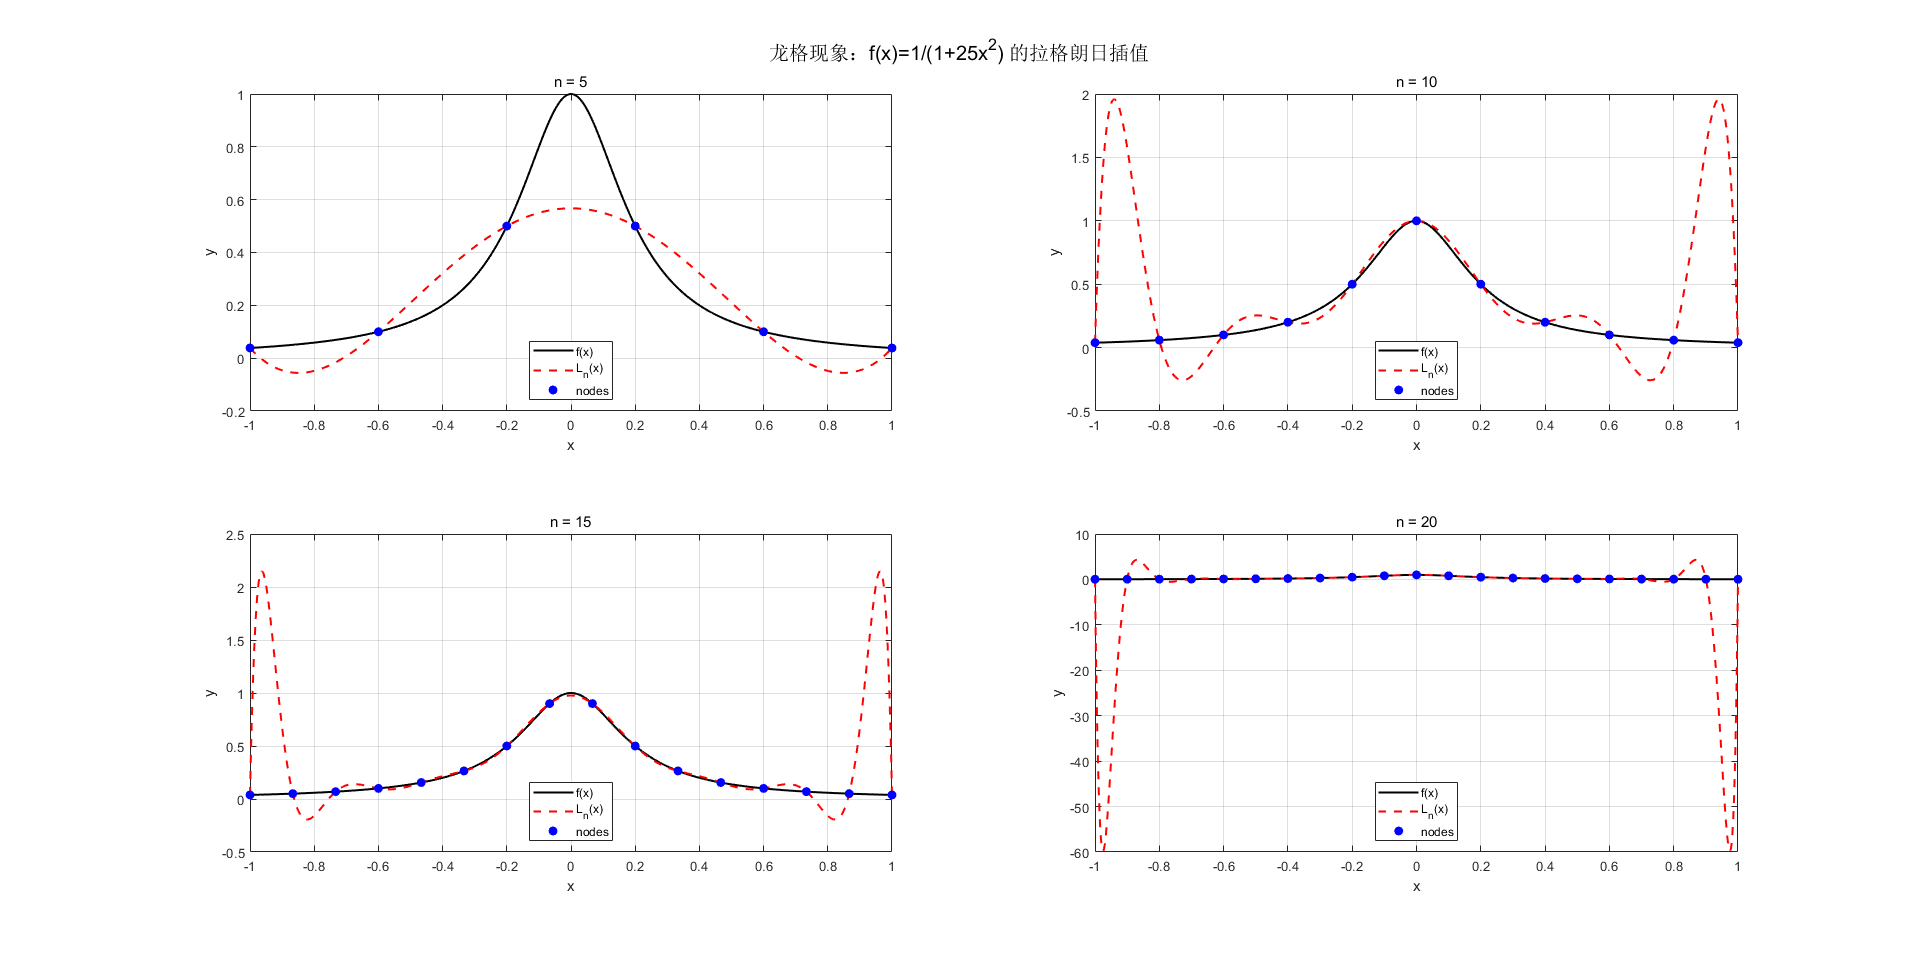
\includegraphics[width=1\linewidth]{figure/2-3-1.png}
    \label{2-3-1}
\end{figure}

可以看出，次数越大，龙格现象越严重，右下角图种函数的相对误差已经有几十了。





\section{实验三}
\subsection*{3.1}
\addcontentsline{toc}{subsection}{3.1}
消去法是我们在数值分析中已经熟悉的。但由于计算机的数值运算是在一个有限的浮点数集合上进行的，如何才能确保 Gauss 消去法作为数值计算法的稳定性呢？Gauss 消去法从理论算法到数值算法，其关键是主元的选择。考虑线性方程组

\[ Ax = b, \quad A \in R^{m \times n}, \, b \in R^m \]

编制一个能自动选取主元，又能手动选取主元的求解线性代数方程组的 Gauss 消元过程。取矩阵

\[ A = \begin{bmatrix} 6 & 1 \\ 8 & 6 & 1 \\ & \ddots & \ddots & \ddots \\ & & 8 & 6 & 1 \\ & & &8  & 6 \end{bmatrix}, \, b = \begin{bmatrix} 7 \\ 15 \\ \vdots \\ 15 \\ 14 \end{bmatrix} \]

则方程有解 \( x^* = (1, 1, \ldots, 1)^T \)。取 m=10 计算矩阵的条件数，让程序自动选取主元，结果如何？

按照题意实现即可。

\begin{lstlisting}[language=matlab]
gauss_elimination_with_pivoting(false)

function gauss_elimination_with_pivoting(auto_pivot)
    m = 10;
    A = zeros(m);
    for i = 1:m
        if i > 1
            A(i,i-1) = 8;
        end
        A(i,i) = 6;
        if i < m
            A(i,i+1) = 1;
        end
    end

    % 设置精确解与对应右端项
    x_true = ones(m,1);
    b = A * x_true;

    % 打印条件数
    fprintf('条件数 cond(A) = %.2e\n', cond(A));

    % 开始Gauss消元
    Ab = [A b];  % 扩展矩阵
    n = m;

    for k = 1:n-1
        % 主元选择
        if auto_pivot
            [~, pivot_row] = max(abs(Ab(k:n,k)));
            pivot_row = pivot_row + k - 1;
        else
            fprintf('当前第 %d 列：\n', k);
            disp(Ab(k:n,k));
            pivot_row = input(['请选择第 ' num2str(k) ' 列的主元行号（从 ' num2str(k) ' 到 ' num2str(n) '）: ']);
        end

        % 行交换
        if pivot_row ~= k
            Ab([k pivot_row], :) = Ab([pivot_row k], :);
        end

        % 消元过程
        for i = k+1:n
            m_ik = Ab(i,k) / Ab(k,k);
            Ab(i,k:end) = Ab(i,k:end) - m_ik * Ab(k,k:end);
        end
    end

    % 回代
    x = zeros(n,1);
    for i = n:-1:1
        x(i) = (Ab(i,end) - Ab(i,i+1:n) * x(i+1:n)) / Ab(i,i);
    end

    % 输出结果
    fprintf('求解误差 ||x - x_true|| = %.2e\n', norm(x - x_true));
end
\end{lstlisting}

某次手动选取主元的运行结果：
\begin{lstlisting}[language=matlab]
条件数 cond(A) = 1.73e+03
求解误差 ||x - x_true|| = 3.84e-14
\end{lstlisting}

自动选取主元的运行结果：
\begin{lstlisting}[language=matlab]
条件数 cond(A) = 1.73e+03
求解误差 ||x - x_true|| = 0.00e+00
\end{lstlisting}

\subsection*{3.2}
\addcontentsline{toc}{subsection}{3.2}
\begin{enumerate}
    \item 判断用 Jacobi 迭代法、Gauss-Seidel 迭代法、SOR 法(分别取 $\omega = 0.8, 1.2, 1.3, 1.6$)解下列线性方程组的收敛性。若收敛，再用 Jacobi 迭代法、Gauss-Seidel 迭代法、SOR 法(分别取 $\omega = 0.8, 1.2, 1.3, 1.6$)分别解线性方程组，并比较各种方法的收敛速度。

\[
\begin{cases}
x_1 - x_2 + 2x_3 + x_4 = 1, \\
-x_1 + 3x_2 - 3x_4 = 3, \\
2x_1 + 9x_3 - 6x_4 = 5, \\
x_1 - 3x_2 - 6x_3 + 19x_4 = 7.
\end{cases}
\]
    \item 用 Cholesky 分解求解下列线性方程组

\[
\begin{bmatrix}
4 & 2 & -4 & 0 & 2 & 4 & 0 & 0 \\
2 & 2 & -1 & -2 & 1 & 3 & 2 & 0 \\
-4 & -1 & 14 & 1 & -8 & -3 & 5 & 6 \\
0 & -2 & 1 & 6 & -1 & -4 & -3 & 3 \\
2 & 1 & -8 & -1 & 22 & 4 & -10 & -3 \\
4 & 3 & -3 & -4 & 4 & 11 & 1 & -4 \\
0 & 2 & 5 & -3 & -10 & 1 & 14 & 2 \\
0 & 0 & 6 & 3 & -3 & -4 & 2 & 19
\end{bmatrix}
\begin{bmatrix}
x_1 \\
x_2 \\
x_3 \\
x_4 \\
x_5 \\
x_6 \\
x_7 \\
x_8 
\end{bmatrix}
=
\begin{bmatrix}
0 \\
-6 \\
6 \\
23 \\
11 \\
-22 \\
-15 \\
45
\end{bmatrix}
\]

(方程组的精确解是 $x^* = (1, -1, 0, 2, 1, -1, 0, 2)^T$.)
\end{enumerate}


给定线性方程组可转化为矩阵形式 $Ax = b$：

$$
A = \begin{bmatrix}
1 & -1 & 2 & 1 \\
-1 & 3 & 0 & -3 \\
2 & 0 & 9 & -6 \\
1 & -3 & -6 & 19
\end{bmatrix}, \quad
b = \begin{bmatrix}
1 \\ 3 \\ 5 \\ 7
\end{bmatrix}
$$


\begin{itemize}
    \item 对于 Jacobi 方法，迭代矩阵为 $T_J = D^{-1}(L + U)$；
    \item 对于 Gauss-Seidel 方法，迭代矩阵为 $T_{GS} = (D - L)^{-1}U$；
    \item 对于 SOR 方法，迭代矩阵为：$T_{SOR} = (D - \omega L)^{-1}[(1 - \omega)D + \omega U]$
\end{itemize}

计算它们的谱半径 $\rho(T)$，若 $\rho < 1$，则对应方法收敛。我们编写matlab程序：
\begin{lstlisting}[language=matlab]
clc; clear;

A = [1, -1, 2, 1;
    -1, 3, 0, -3;
     2, 0, 9, -6;
     1, -3, -6, 19];

D = diag(diag(A));
L = tril(A, -1);
U = triu(A, 1);

% Jacobi
T_jacobi = -D \ (L + U);
rho_jacobi = max(abs(eig(T_jacobi)));

% Gauss-Seidel
T_gs = -(D - L) \ U;
rho_gs = max(abs(eig(T_gs)));

% SOR for various ω
omegas = [0.8, 1.2, 1.3, 1.6];
rho_sor = zeros(size(omegas));

for i = 1:length(omegas)
    omega = omegas(i);
    T_sor = inv(D - omega * L) * ((1 - omega) * D + omega * U);
    rho_sor(i) = max(abs(eig(T_sor)));
end

% 输出
fprintf("Jacobi 收敛性判断：rho = %.4f ⇒ %s\n", rho_jacobi, verdict(rho_jacobi));
fprintf("Gauss-Seidel 收敛性判断：rho = %.4f ⇒ %s\n", rho_gs, verdict(rho_gs));

for i = 1:length(omegas)
    fprintf("SOR(ω = %.1f) 收敛性判断：rho = %.4f ⇒ %s\n", omegas(i), rho_sor(i), verdict(rho_sor(i)));
end

% 帮助函数
function result = verdict(rho)
    if rho < 1
        result = "收敛";
    else
        result = "不收敛";
    end
end
\end{lstlisting}

\begin{lstlisting}[language=matlab]
Jacobi 收敛性判断：rho = 0.9669 ⇒ 收敛
Gauss-Seidel 收敛性判断：rho = 0.8156 ⇒ 收敛
SOR(ω = 0.8) 收敛性判断：rho = 0.8765 ⇒ 收敛
SOR(ω = 1.2) 收敛性判断：rho = 0.7179 ⇒ 收敛
SOR(ω = 1.3) 收敛性判断：rho = 0.6339 ⇒ 收敛
SOR(ω = 1.6) 收敛性判断：rho = 0.6119 ⇒ 收敛
\end{lstlisting}
故这些方法都收敛。
\begin{lstlisting}[language=matlab]
function iter_solve_all()
    % 系数矩阵 A 与 右端向量 b
    A = [ 1  -1   2   1;
         -1   3   0  -3;
          2   0   9  -6;
          1  -3  -6  19];
    b = [1; 3; 5; 7];
    x_true = A\b;

    % Jacobi
    fprintf("=== Jacobi ===\n");
    [x_jacobi, iter_j] = iter_solve(A, b, 'jacobi');

    % Gauss-Seidel
    fprintf("=== Gauss-Seidel ===\n");
    [x_gs, iter_gs] = iter_solve(A, b, 'gs');

    % SOR for different omega
    omega_list = [0.8, 1.2, 1.3, 1.6];
    iter_sor = zeros(size(omega_list));
    for i = 1:length(omega_list)
        omega = omega_list(i);
        fprintf("=== SOR (omega = %.1f) ===\n", omega);
        [x_sor, iter_sor(i)] = iter_solve(A, b, 'sor', omega);
    end

    % 输出比较
    fprintf("\n=== 总结 ===\n");
    fprintf("方法\t\t迭代次数\n");
    fprintf("Jacobi\t\t%d\n", iter_j);
    fprintf("Gauss-Seidel\t%d\n", iter_gs);
    for i = 1:length(omega_list)
        fprintf("SOR (w=%.1f)\t%d\n", omega_list(i), iter_sor(i));
    end
end

% ---------- 核心迭代函数 ----------
function [x, iter] = iter_solve(A, b, method, omega)
    if nargin < 4
        omega = 1.0;
    end

    n = length(b);
    x = zeros(n,1);   % 初始解
    tol = 1e-6;
    max_iter = 1000;
    iter = 0;

    D = diag(diag(A));
    L = tril(A,-1);
    U = triu(A,1);

    switch lower(method)
        case 'jacobi'
            B = -inv(D) * (L + U);
            c = inv(D) * b;
        case 'gs'
            B = -inv(D+L) * U;
            c = inv(D+L) * b;
        case 'sor'
            B = inv(D + omega*L) * ((1 - omega)*D - omega*U);
            c = omega * inv(D + omega*L) * b;
        otherwise
            error('Unknown method');
    end

    % 判断收敛性
    rho = max(abs(eig(B)));
    fprintf('谱半径 rho = %.4f\n', rho);
    if rho >= 1
        fprintf('不收敛（rho ≥ 1）\n');
        return;
    else
        fprintf('满足收敛条件（rho < 1）\n');
    end

    % 开始迭代
    while iter < max_iter
        x_new = B * x + c;
        if norm(x_new - x, inf) < tol
            break;
        end
        x = x_new;
        iter = iter + 1;
    end
    fprintf('收敛于 %d 步，误差 = %.2e\n\n', iter, norm(A*x - b));
end
\end{lstlisting}


输出样例（含收敛性分析）
\begin{lstlisting}[language=matlab]
=== Jacobi ===
谱半径 rho = 0.9669
满足收敛条件（rho < 1）
收敛于 377 步，误差 = 3.82e-06

=== Gauss-Seidel ===
谱半径 rho = 0.9349
满足收敛条件（rho < 1）
收敛于 200 步，误差 = 1.28e-06

=== SOR (omega = 0.8) ===
谱半径 rho = 0.9565
满足收敛条件（rho < 1）
收敛于 293 步，误差 = 1.99e-06

=== SOR (omega = 1.2) ===
谱半径 rho = 0.9019
满足收敛条件（rho < 1）
收敛于 135 步，误差 = 1.06e-06

=== SOR (omega = 1.3) ===
谱半径 rho = 0.8775
满足收敛条件（rho < 1）
收敛于 109 步，误差 = 1.03e-06

=== SOR (omega = 1.6) ===
谱半径 rho = 0.6089
满足收敛条件（rho < 1）
收敛于 34 步，误差 = 1.38e-06


=== 总结 ===
方法		迭代次数
Jacobi		377
Gauss-Seidel	200
SOR (w=0.8)	293
SOR (w=1.2)	135
SOR (w=1.3)	109
SOR (w=1.6)	34
\end{lstlisting}

结论总结：

该系统对 Jacobi 和 Gauss-Seidel 都 收敛（谱半径均 < 1）。
Gauss-Seidel 明显 比 Jacobi 更快。
SOR 最快的 $\omega$ 值是 $1.6$。收敛越快的 $\omega$ 值，谱半径更小。

(2) 用 Cholesky 分解求解线性方程组

方法：

设线性方程组为
\[
Ax = b,
\]
其中 \(A \in \mathbb{R}^{n \times n}\) 是对称正定矩阵，\(x, b \in \mathbb{R}^n\)。

由于 \(A\) 是对称正定矩阵，存在唯一的下三角矩阵 \(L\)，满足
\[
A = LL^\top.
\]

将分解代入原方程，有
\[
LL^\top x = b.
\]

令
\[
L^\top x = y,
\]
则有
\[
Ly = b.
\]

先通过前向替代求解下三角线性方程
\[
Ly = b,
\]
得到中间变量 \(y\)。

再通过后向替代求解上三角线性方程
\[
L^\top x = y,
\]
从而得到最终解 \(x\)。

综上，通过 Cholesky 分解 \(A = LL^\top\)，可将原方程 \(Ax = b\) 转化为两个三角方程，依次求解可得解向量 \(x\)。

\begin{lstlisting}[language=matlab]
A=[
4  2  -4  0  2  4  0  0 ;
2  2  -1  -2  1  3  2  0 ;
-4  -1  14  1  -8  -3  5  6;
0  -2  1  6  -1  -4  -3  3;
2  1  -8  -1  22  4  -10  -3;
4  3  -3  -4  4  11  1  -4;
0  2  5  -3  -10  1  14  2;
0  0  6  3  -3  -4  2  19];
b=[0 ;-6 ;6 ;23 ;11 ;-22 ;-15 ;45];
L = chol(A, 'lower');
y = L \ b;
x = L' \ y;
x_exact=[1, -1, 0, 2, 1, -1, 0, 2]';
fprintf('误差 ‖x - x_exact‖ = %.2e\n', norm(x - x_exact));
\end{lstlisting}

\begin{lstlisting}[language=matlab]
误差 ‖x - x_exact‖ = 0.00e+00
\end{lstlisting}

\subsection*{3.3}
\addcontentsline{toc}{subsection}{3.3}
设
\[ A = \begin{bmatrix} 20 & 2 & 3 \\ 1 & 8 & 1 \\ 2 & -3 & 15 \end{bmatrix}, \quad b_1 = \begin{bmatrix} 1 \\ 0 \\ 0 \end{bmatrix}, \quad b_2 = \begin{bmatrix} 0 \\ 1 \\ 0 \end{bmatrix}, \quad b_3 = \begin{bmatrix} 0 \\ 0 \\ 1 \end{bmatrix} \]

\begin{enumerate}
    \item 将矩阵 A 进行 LU 分解，$A = LU$，其中 U 是上三角矩阵，L 是主对角线上的元素都是 1 的下三角矩阵。
    \item 利用上述分解分别求解方程组
\[ AX = b_1, \quad AX = b_2, \quad AX = b_3 \]
并由此求出逆矩阵 $A^{-1}$。
    \item 用 LU 分解求下列线性方程组的解


\[
\begin{bmatrix}
4 & 2 & -3 & -1 & 2 & 1 & 0 & 0 & 0 & 0  \\
8 & 6 & -5 & -3 & 6 & 5 & 0 & 1 & 0 & 0  \\
4 & 2 & -2 & -1 & 3 & 2 & -1 & 0 & 3 & 1 \\
0 & -2 & 1 & 5 & -1 & 3 & -1 & 1 & 9 & 4 \\
-4 & 2 & 6 & -1 & 6 & 7 & -3 & 3 & 2 & 3 \\
8 & 6 & -8 & 5 & 7 & 17 & 2 & 6 & -3 & 5 \\
0 & 2 & -1 & 3 & -4 & 2 & 5 & 3 & 0 & 1 \\
16 & 10 & -11 & -9 & 17 & 34 & 2 & -1 & 2 & 2 \\
4 & 6 & 2 & -7 & 13 & 9 & 2 & 0 & 12 & 4 \\
0 & 0 & -1 & 8 & -3 & -24 & -8 & 6 & 3 & -1 
\end{bmatrix}
\begin{bmatrix}
x_1 \\
x_2 \\
x_3 \\
x_4 \\
x_5 \\
x_6 \\
x_7 \\
x_8 \\
x_9 \\
x_{10}
\end{bmatrix}
=
\begin{bmatrix}
5 \\
12 \\
3 \\
2 \\
3 \\
46 \\
13 \\
38 \\
19 \\
-21
\end{bmatrix}
\]

（方程组的精确解是 $x^* = (1, -1, 0, 1, 2, 0, 3, 1, -1, 2)^T$.）
\end{enumerate}

\begin{lstlisting}[language=matlab]
% (1) LU 分解 A = LU，其中 L 单位下三角矩阵，U 上三角
A = [20 2 3; 1 8 1; 2 -3 15];
n = size(A,1);
L = eye(n);
U = zeros(n);

for k = 1:n
    U(k,k:n) = A(k,k:n) - L(k,1:k-1)*U(1:k-1,k:n);
    for i = k+1:n
        L(i,k) = (A(i,k) - L(i,1:k-1)*U(1:k-1,k)) / U(k,k);
    end
end

disp('L ='); disp(L);
disp('U ='); disp(U);
\end{lstlisting}

\begin{lstlisting}[language=matlab]
L =
                         1                         0                         0
                      0.05                         1                         0
                       0.1        -0.405063291139241                         1

U =
                        20                         2                         3
                         0                       7.9                      0.85
                         0                         0          15.0443037974684
\end{lstlisting}

\begin{lstlisting}[language=matlab]
% 三个右端项向量
b1 = [1; 0; 0];
b2 = [0; 1; 0];
b3 = [0; 0; 1];

% 求 Ax = b1
y1 = L \ b1;
x1 = U \ y1;

% 求 Ax = b2
y2 = L \ b2;
x2 = U \ y2;

% 求 Ax = b3
y3 = L \ b3;
x3 = U \ y3;

disp('A^{-1} ='); disp([x1,x2,x3]);
disp('验证 A * A^{-1} = I:'); disp(A * [x1,x2,x3]);
\end{lstlisting}

\begin{lstlisting}[language=matlab]
A^{-1} =
        0.0517458981909971       -0.0164072360117796      -0.00925536390408077
      -0.00546907867059318         0.123685317627261      -0.00715187210769878
      -0.00799326882625158        0.0269246949936895         0.066470340765671

验证 A * A^{-1} = I:
                         1      2.77555756156289e-17                         0
     -6.93889390390723e-18                         1                         0
     -2.77555756156289e-17      5.55111512312578e-17                         1
\end{lstlisting}

\begin{lstlisting}[language=matlab]
% (3) 解10x10线性方程组 Ax = b
A = [4 2 -3 -1 2 1 0 0 0 0;
     8 6 -5 -3 6 5 0 1 0 0;
     4 2 -2 -1 3 2 -1 0 3 1;
     0 -2 1 5 -1 3 -1 1 9 4;
    -4 2 6 -1 6 7 -3 3 2 3;
     8 6 -8 5 7 17 2 6 -3 5;
     0 2 -1 3 -4 2 5 3 0 1;
    16 10 -11 -9 17 34 2 -1 2 2;
     4 6 2 -7 13 9 2 0 12 4;
     0 0 -1 8 -3 -24 -8 6 3 -1];
b = [5;12;3;2;3;46;13;38;19;-21];
x_true = [1; -1; 0; 1; 2; 0; 3; 1; -1; 2];

% LU 分解（带行置换）
[L,U,P] = lu(A);

% 解 Ly = Pb
y = L \ (P * b);

% 解 Ux = y
x = U \ y;

% 输出与误差
disp('解 x ='); disp(x);
fprintf('误差 ‖x - x_true‖ = %.2e\n', norm(x - x_true));
\end{lstlisting}
\begin{lstlisting}[language=matlab]
解 x =
          1.00000000000002
         -1.00000000000003
      1.37820789263813e-14
         0.999999999999989
                         2
      1.36748024588164e-16
                         3
          1.00000000000002
                        -1
                         2

误差 ‖x - x_true‖ = 4.50e-14
\end{lstlisting}


\subsection*{3.4}
\addcontentsline{toc}{subsection}{3.4}
\begin{enumerate}
    \item 用追赶法求解方程组 $AX = b$
    \begin{enumerate}
        \item $A = \begin{bmatrix}
4 & 1 \\
1 & 4 & 1 \\
&\ddots & \ddots & \ddots \\
&1 & 4 & 1 \\
& &1 & 4 
\end{bmatrix}_{30 \times 30}, \quad 
b = \begin{bmatrix}
2 \\
1 \\
\vdots \\
1 \\
2
\end{bmatrix}_{30 \times 1}$
        \item $A = \begin{bmatrix} 5 & -2 & 1 \\ -2 & 5 & -2 & 1 \\ 1 & -2 & 5 & -2 & 1 \\
& \ddots & \ddots & \ddots & \ddots & \ddots \\
& &1 & -2 & 5 & -2 & 1 \\
& & &1 & -2 & 5 & -2 \\
&&&&1 &-2 &5
\end{bmatrix}_{20 \times 20}, \quad b = \begin{bmatrix} 1 \\ 0 \\ 0 \\ \vdots \\ 0 \\ 0 \end{bmatrix}_{20 \times 1}$
    \end{enumerate}
    \item 设计实验验证 Hilbert 矩阵 $H_n$ 的病态性，其中

\[ H_n = \begin{pmatrix}
1 & \frac{1}{2} & \cdots & \frac{1}{n} \\
\frac{1}{2} & \frac{1}{3} & \cdots & \frac{1}{n+1} \\
\vdots & \vdots & \ddots & \vdots \\
\frac{1}{n} & \frac{1}{n+1} & \cdots & \frac{1}{2n-1}
\end{pmatrix}.
\]
\end{enumerate}

三对角线追赶法：

设线性方程组为
\[
Ax = b,
\]
其中 \(A\) 是一个 \(n \times n\) 的严格三对角矩阵，即只有主对角线、下对角线和上对角线非零，具体表示为：

\[
A = 
\begin{bmatrix}
b_1 & c_1 &        &        &  \\
a_2 & b_2 & c_2    &        &  \\
    & a_3 & b_3    & \ddots &  \\
    &     & \ddots & \ddots & c_{n-1} \\
    &     &        & a_n    & b_n
\end{bmatrix}, \quad
x = 
\begin{bmatrix}
x_1 \\
x_2 \\
\vdots \\
x_n
\end{bmatrix}, \quad
b = 
\begin{bmatrix}
d_1 \\
d_2 \\
\vdots \\
d_n
\end{bmatrix}.
\]

引入修改后的系数：
\[
\tilde{c}_1 = \frac{c_1}{b_1}, \quad
\tilde{d}_1 = \frac{d_1}{b_1}.
\]

对 \(i = 2,3,\ldots,n\)，递推定义：
\[
\tilde{c}_i = 
\begin{cases}
\frac{c_i}{b_i - a_i \tilde{c}_{i-1}}, & i < n, \\
\text{不需要定义}, & i = n,
\end{cases}
\quad
\tilde{d}_i = \frac{d_i - a_i \tilde{d}_{i-1}}{b_i - a_i \tilde{c}_{i-1}}.
\]

完成上述递推后，使用回代求解 \(x_n, x_{n-1}, \ldots, x_1\)：

\[
x_n = \tilde{d}_n,
\quad
x_i = \tilde{d}_i - \tilde{c}_i x_{i+1}, \quad i = n-1, n-2, \ldots, 1.
\]

因此，通过两轮迭代（一次前向，计算 \(\tilde{c}_i, \tilde{d}_i\)，一次回代，计算 \(x_i\)），可在线性时间内求解三对角线性系统。


\begin{enumerate}
    \item 
    \begin{lstlisting}[language=matlab]
n1 = 30;
a1 = ones(n1-1,1);    % 下对角线
b1 = 4*ones(n1,1);    % 主对角线
c1 = ones(n1-1,1);    % 上对角线

d1 = ones(n1,1);
d1(1) = 2; d1(end) = 2;

x1 = tridiag_solver(a1, b1, c1, d1);
disp('第一个方程组解 x1 =');
disp(x1);



function x = tridiag_solver(a, b, c, d)
% 追赶法解三对角线性方程组 Ax=d
% a: 下对角线元素，长度 n-1
% b: 主对角线元素，长度 n
% c: 上对角线元素，长度 n-1
% d: 右端项，长度 n

n = length(b);
% 初始化临时向量
c_prime = zeros(n-1,1);
d_prime = zeros(n,1);

% 前向消元
c_prime(1) = c(1) / b(1);
d_prime(1) = d(1) / b(1);
for i=2:n-1
    denom = b(i) - a(i-1)*c_prime(i-1);
    c_prime(i) = c(i) / denom;
    d_prime(i) = (d(i) - a(i-1)*d_prime(i-1)) / denom;
end
d_prime(n) = (d(n) - a(n-1)*d_prime(n-1)) / (b(n) - a(n-1)*c_prime(n-1));

% 回代
x = zeros(n,1);
x(n) = d_prime(n);
for i=n-1:-1:1
    x(i) = d_prime(i) - c_prime(i)*x(i+1);
end
end
    \end{lstlisting}
\begin{lstlisting}[language=matlab]
第一个方程组解 x1 =
          0.47927405783631
        0.0829037686547607
         0.189110867544647
          0.16065276116665
         0.168278087788752
         0.166234887678343
         0.166782361497876
         0.166635666330151
         0.166674973181518
         0.166664440943776
         0.166667263043376
         0.166666506882718
         0.166666709425752
         0.166666655414276
         0.166666668917145
         0.166666668917145
         0.166666655414276
         0.166666709425752
         0.166666506882718
         0.166667263043376
         0.166664440943776
         0.166674973181518
         0.166635666330151
         0.166782361497876
         0.166234887678343
         0.168278087788752
          0.16065276116665
         0.189110867544647
        0.0829037686547608
          0.47927405783631
\end{lstlisting}
\begin{lstlisting}[language=matlab]
% 定义矩阵大小
n = 20;

% 初始化矩阵 A 和向量 b
A = zeros(n, n);
b = zeros(n, 1);
b(1) = 1; % b 的第一个元素为 1，其余为 0

% 填充矩阵 A 的五对角元素
for i = 1:n
    A(i, i) = 5; % 主对角线
    if i > 1
        A(i, i-1) = -2; % 下对角线（紧邻主对角线）
    end
    if i < n
        A(i, i+1) = -2; % 上对角线（紧邻主对角线）
    end
    if i > 2
        A(i, i-2) = 1; % 下对角线（再往外）
    end
    if i < n-1
        A(i, i+2) = 1; % 上对角线（再往外）
    end
end

% LU 分解（针对五对角矩阵）
L = eye(n); % L 初始化为主对角线为 1 的矩阵
U = zeros(n, n); % U 初始化为零矩阵

% 第一行直接赋值
U(1, 1) = A(1, 1);
U(1, 2) = A(1, 2);
U(1, 3) = A(1, 3);

% 计算 L 和 U 的元素
for i = 2:n
    % 计算 L 的下三角元素
    L(i, i-1) = A(i, i-1) / U(i-1, i-1); % 紧邻下对角线
    if i > 2
        L(i, i-2) = (A(i, i-2) - L(i, i-1) * U(i-1, i-2)) / U(i-2, i-2); % 再往外的下对角线
    end
    
    % 计算 U 的上三角元素
    U(i, i) = A(i, i) - L(i, i-1) * U(i-1, i);
    if i > 2
        U(i, i) = U(i, i) - L(i, i-2) * U(i-2, i);
    end
    if i < n
        U(i, i+1) = A(i, i+1) - L(i, i-1) * U(i-1, i+1);
    end
    if i < n-1
        U(i, i+2) = A(i, i+2);
    end
end

% 前代法求解 Ly = b
y = zeros(n, 1);
y(1) = b(1);
for i = 2:n
    y(i) = b(i) - L(i, i-1) * y(i-1);
    if i > 2
        y(i) = y(i) - L(i, i-2) * y(i-2);
    end
end

% 回代法求解 Ux = y
x = zeros(n, 1);
x(n) = y(n) / U(n, n);
x(n-1) = (y(n-1) - U(n-1, n) * x(n)) / U(n-1, n-1);
for i = n-2:-1:1
    x(i) = (y(i) - U(i, i+1) * x(i+1) - U(i, i+2) * x(i+2)) / U(i, i);
end

% 显示结果
disp('解向量 x 为：');
disp(x);

% 验证解的正确性
residual = A * x - b;
disp('残差 norm(Ax - b) 为：');
disp(norm(residual));
\end{lstlisting}
\begin{lstlisting}[language=matlab]
解向量 x 为：
         0.241446913591857
        0.0983223881384271
       -0.0105897916824291
       -0.0298976968732801
       -0.0123196173940466
       0.00131307171981118
       0.00373647858222237
       0.00153998907419014
     -0.000164123793491864
     -0.000467059185673314
     -0.000192498607148396
      2.05155238489456e-05
      5.83822541353113e-05
       2.4061878330607e-05
     -2.56453763795259e-06
     -7.29613715970092e-06
     -3.00487922614044e-06
      3.18272125407045e-07
      8.97152265140598e-07
      3.62492900860381e-07

残差 norm(Ax - b) 为：
         0.041404213307586
\end{lstlisting}
    \item
\begin{lstlisting}[language=matlab]
% 计算 Hilbert 矩阵及其条件数
n_vals = [5, 8, 12, 15, 20];
fprintf('n\tcond(H_n)\n');
for n = n_vals
    H = hilb(n);
    cond_H = cond(H);
    fprintf('%d\t%e\n', n, cond_H);
end

% 观察随着 n 增大，条件数指数增长，矩阵越来越病态
\end{lstlisting}
\begin{lstlisting}[language=matlab]
n	cond(H_n)
5	4.766073e+05
8	1.525758e+10
12	1.621164e+16
15	2.495952e+17
20	2.106531e+18
\end{lstlisting}
\end{enumerate}
\section{实验四}
\subsection*{4.1}
\addcontentsline{toc}{subsection}{4.1}
分别用下列方法计算积分 $I = \int_0^1 \frac{xe^x}{(1+x)^2} dx$，

\begin{enumerate}
    \item Romberg 算法；
    
    设 $T_{m,1}$ 是用步长 $h_m = \frac{b-a}{2^{m-1}}$ 的复化梯形公式结果：

    $$
    T_{m,1} = \text{复化梯形公式},\quad m = 1, 2, \dots
    $$

    然后用递推公式计算高阶逼近：
    
    $$
    T_{m,k} = \frac{4^{k-1} T_{m,k-1} - T_{m-1,k-1}}{4^{k-1} - 1}, \quad k = 2,3,\dots,m
    $$

    Romberg 算法最终结果是 $T_{m,m}$，即误差阶为 $O(h^{2m})$ 的高精度近似。
\begin{lstlisting}[language=matlab]
f = @(x) (x .* exp(x)) ./ (1 + x).^2;
a = 0;
b = 1;
m = 10;
I = romberg_core(f, a, b, m);
fprintf('Romberg 积分结果 I = %.10f\n', I);


function I = romberg_core(f, a, b, m)
    R = zeros(m, m);
    for k = 1:m
        n = 2^(k-1);
        h = (b - a)/n;
        x = linspace(a, b, n+1);
        R(k,1) = h * (0.5*f(a) + sum(f(x(2:end-1))) + 0.5*f(b));  % T_{k,1}
    end

    for j = 2:m
        for k = j:m
            R(k,j) = (4^(j-1)*R(k,j-1) - R(k-1,j-1)) / (4^(j-1) - 1);
        end
    end

    I = R(m,m);
end
\end{lstlisting}

\begin{lstlisting}[language=matlab]
I_romberg = 0.359140910232952
\end{lstlisting}
    \item 8 点 Gauss 公式；

我们的积分估计形如$\int_a^bf(x)\mathrm{d}x=\sum_{i=1}^n A_i f(x_i)$。可以证明八次勒让德多项式的零点即为高斯点（$x_i$），相应的权重（$A_i$）为常数。我们将它们从$[-1,1]$映射到$[a,b]$即可。
\begin{lstlisting}[language=matlab]
% 定义被积函数（变换后）
f = @(t) (t + 1) ./ (2 * (t + 3).^2) .* exp((t + 1));
% 8点Gauss-Legendre节点和权重（高精度值）
nodes = [-0.9602898564975363; -0.7966664774136267; -0.5255324099163290; 
         -0.1834346424956498;  0.1834346424956498;  0.5255324099163290;
          0.7966664774136267;  0.9602898564975363];
      
weights = [0.1012285362903763; 0.2223810344533745; 0.3137066458778873;
           0.3626837833783620; 0.3626837833783620; 0.3137066458778873;
           0.2223810344533745; 0.1012285362903763];

% 计算积分近似值
I_approx = sum(weights .* f(nodes));
% 显示结果
fprintf('8点Gauss公式近似值: %.15f\n', I_approx);
\end{lstlisting}
    \item 将积分区间分为 5 等份，用复化两点 Gauss 公式即为把区间分为若干份，对每个区间使用高斯两点公式。；并比较结果。
    
    复化两点 Gauss 公式即为把区间分为若干份，对每个区间使用高斯两点公式。
\begin{lstlisting}[language=matlab]
f = @(x) x .* exp(x) ./ (1 + x).^2;
a = 0; b = 1; n = 5;
h = (b - a) / n;
I_comp = 0;
for i = 0:n-1
    x0 = a + i*h;
    x1 = x0 + h;
    m = (x0 + x1)/2;  % 中点
    r = h/2;
    % 两点 Gauss 节点 & 权重（标准 [-1,1]）
    x1_gauss = m - r/sqrt(3);
    x2_gauss = m + r/sqrt(3);
    I_comp = I_comp + r * (f(x1_gauss) + f(x2_gauss));
end
\end{lstlisting}
\begin{lstlisting}[language=matlab]
I_comp = 0.359143879148435
\end{lstlisting}
\end{enumerate}



\subsection*{4.2}
\addcontentsline{toc}{subsection}{4.2}
设某城市男子的身高 $X\sim \mathcal{N}(170, 36)$（单位：cm），应如何选择公共汽车门的高度 $H$ 使男子与车门碰头的机会小于 $1\%$。

问题分析：由题设男子身高数据服从平均值为 $170$（cm），方差为 $6$（cm）的正态分布，其分布密度函数为

\[ f(x) = \frac{1}{6\sqrt{2\pi}} \exp\left[-\frac{(x-170)^2}{2 \times 36}\right] \]

按正态分布的分布规律，这个城市的男子身高超过 188（cm）的人数极少。故可以对 $H=188, 187, 186, \dots$ 求出概率 $P(X > H)$ 的值，观察使概率不超过 $1\%$ 的 $H$，以确定公共汽车门应该取的高度。概念值的计算实际上是求定积分

\[ P\{X > H\} = \int_{H}^{+\infty} f(x) dx \approx \int_{H}^{194} f(x) dx \]

(1) 选用一种数值求积公式或用数学软件分别计算出 $H=180, 181, …, 188$ 时定积分近似值。

(2) 根据上面计算的积分值，按题目要求确定公共车门的高度取值（答案 $184$cm）。如果将汽车门的高度取 $180$cm，是否满足大多数市民的利益？

(3) 用计算机模拟的方法来检验你的结论，计算机产生 $10000$ 个正态随机数（它们服从均值为 $170$，方差为 $6$ 的正态分布）来模拟这个城市中 $10000$ 个男子的身高，然后统计出这 $10000$ 人中身高超过 $180$cm的男子数量所占的百分比。

\begin{lstlisting}[language=matlab]
% 参数设置
mu = 170;
sigma = sqrt(36);  % 标准差 = 6

% (1) 分析 H = 180 到 188 时 P(X > H)
H_vals = 180:188;
P_vals = arrayfun(@(H) integral(@(x) normpdf(x, mu, sigma), H, Inf), H_vals);

% (2) 找出第一个满足 P(X > H) < 0.01 的 H
H_threshold = H_vals(find(P_vals < 0.01, 1));

% (3) 模拟法：生成 10000 个正态样本，统计 >180 的比例
samples = normrnd(mu, sigma, [10000, 1]);
percentage_over_180 = mean(samples > 180) * 100;

% 显示结果
disp('H 值范围:');
disp(H_vals);
disp('对应的 P(X > H):');
disp(round(P_vals, 5));
disp(['使 P(X > H) < 0.01 的最小 H: ', num2str(H_threshold)]);
disp(['模拟中大于 180 的样本比例: ', num2str(percentage_over_180, '%.2f'), '%']);
\end{lstlisting}

\begin{lstlisting}[language=matlab]
H 值范围:
   180   181   182   183   184   185   186   187   188

对应的 P(X > H):
0.04779 0.03338 0.02275 0.01513 0.00982 0.00621 0.00383 0.0023 0.00135

使 P(X > H) < 0.01 的最小 H: 184
模拟中大于 180 的样本比例: 4.47%
\end{lstlisting}

\subsection*{4.3}
\addcontentsline{toc}{subsection}{4.3}
测得定积分 $I = \int_0^2 f(x) dx$ 中被积函数 $Y = f(x)$ 在积分变量 $x$ 的某几个特定点 $X = 0, 0.1571, 0.4712, 0.5498, 0.628, 0.8639, 1.0210, 1.0996, 1.5708$ 处的值分别为 $Y = 0, 0.1565, 0.4540, 0.5225, 0.5878, 0.7604, 0.8526, 0.8910, 1.0000$，试根据这些值首先分别用分段二、三阶拉格朗日插值多项式和三次样条插值函数构造被积函数，然后分别用 \verb|quad| 函数和 \verb|quad8| 函数计算，取精度为 $10^{-4}$，并将计算结果与精确值 $1$ 进行比较。

\begin{lstlisting}[language=matlab]
clc; clear;

% 给定数据点
X = [0, 0.1571, 0.4712, 0.5498, 0.628, 0.8639, 1.0210, 1.0996, 1.5708];
Y = [0, 0.1565, 0.4540, 0.5225, 0.5878, 0.7604, 0.8526, 0.8910, 1.0000];

% 目标积分区间
a = 0; b = 2;
I_exact = 1; % 精确值

lagrange2 = @(x) piecewise_lagrange_interp(x, X, Y, 2);
lagrange3 = @(x) piecewise_lagrange_interp(x, X, Y, 3);
spline_interp = @(x) spline(X, Y, x);

%% 设置积分选项，精度1e-4
opts = optimset('TolFun',1e-4);

%% 计算积分

% 对分段二阶拉格朗日插值函数积分
I_lag2_quad = quad(lagrange2, a, b, 1e-4);
I_lag2_quadl = quadl(lagrange2, a, b, 1e-4);

% 对分段三阶拉格朗日插值函数积分
I_lag3_quad = quad(lagrange3, a, b, 1e-4);
I_lag3_quadl = quadl(lagrange3, a, b, 1e-4);

% 对三次样条插值函数积分
I_spline_quad = quad(spline_interp, a, b, 1e-4);
I_spline_quadl = quadl(spline_interp, a, b, 1e-4);

%% 输出结果及误差

fprintf('方法                | quad积分结果 | 误差        | quadl积分结果 | 误差\n');
fprintf('---------------------|--------------|-------------|---------------|-----------\n');
fprintf('分段二阶拉格朗日     | %.6f     | %.6e | %.6f      | %.6e\n', I_lag2_quad, abs(I_lag2_quad - I_exact), I_lag2_quadl, abs(I_lag2_quadl - I_exact));
fprintf('分段三阶拉格朗日     | %.6f     | %.6e | %.6f      | %.6e\n', I_lag3_quad, abs(I_lag3_quad - I_exact), I_lag3_quadl, abs(I_lag3_quadl - I_exact));
fprintf('三次样条插值         | %.6f     | %.6e | %.6f      | %.6e\n', I_spline_quad, abs(I_spline_quad - I_exact), I_spline_quadl, abs(I_spline_quadl - I_exact));



%% --- 分段拉格朗日插值辅助函数 --- %%
function val = piecewise_lagrange_interp(x, X, Y, order)
    % order: 2代表二阶（三点），3代表三阶（四点）
    % X,Y为数据点，x为待插值点向量或标量
    val = zeros(size(x));
    n = length(X);

    for k = 1:length(x)
        xi = x(k);
        % 找到xi所在区间索引
        idx = find(X <= xi, 1, 'last');
        if isempty(idx) || idx == n
            idx = n-1; % 边界处理，防止超出索引
        end

        % 确定插值点索引范围
        if order == 2
            % 用3个点，尽量选idx-1, idx, idx+1
            inds = idx-1:idx+1;
            if inds(1) < 1
                inds = inds + 1;
            elseif inds(end) > n
                inds = inds - 1;
            end
        elseif order == 3
            % 用4个点，idx-1:idx+2
            inds = idx-1:idx+2;
            if inds(1) < 1
                inds = inds + (2 - inds(1));
            elseif inds(end) > n
                inds = inds - (inds(end) - n);
            end
        else
            error('仅支持order=2或3');
        end

        % 拉格朗日插值多项式计算
        x_nodes = X(inds);
        y_nodes = Y(inds);
        Lk = zeros(1,length(inds));
        for i=1:length(inds)
            % 计算第i个基函数
            Li = 1;
            for j=1:length(inds)
                if j ~= i
                    Li = Li * (xi - x_nodes(j)) / (x_nodes(i) - x_nodes(j));
                end
            end
            Lk(i) = Li;
        end
        val(k) = sum(Lk .* y_nodes);
    end
end
\end{lstlisting}

\begin{lstlisting}[language=matlab]
方法                | quad积分结果 | 误差        | quadl积分结果 | 误差
分段二阶拉格朗日     | 1.417330     | 4.173297e-01 | 1.417384      | 4.173843e-01
分段三阶拉格朗日     | 1.413640     | 4.136405e-01 | 1.413593      | 4.135925e-01
三次样条插值         | 1.414388     | 4.143879e-01 | 1.414301      | 4.143005e-01
\end{lstlisting}

\verb|quad8|函数在\verb|MatlabR2022b|已经不存在了，我使用了\verb|quadl|替代它。

\subsection*{4.4}
\addcontentsline{toc}{subsection}{4.4}
\begin{enumerate}
    \item 用梯形公式、辛普森和牛顿-科茨求积公式计算定积分 $I = \int_0^{\pi/2} e \sin x ^{\sin x} \mathrm{d} x$，取精度 $10^{-4}$，做出它们的积分图并与精确值进行比较；
    \item 用高斯-勒让德积分公式计算 $I = \frac{1}{\sqrt{2\pi}} \int_{-1}^1 e^{-\frac{x^2}{2}} dx$，取代数精度为 3 和 5，再根据截断误差公式写出误差公式，并将计算结果与精确值进行比较。
\end{enumerate}

\begin{enumerate}
\item 用梯形公式、辛普森公式、牛顿-科茨公式计算

\begin{itemize}
    \item 梯形公式：$I = \int_a^{b} f(x) \mathrm{d} x \approx \frac{f(a)+f(b)}{2}(b-a)$；
    \item 辛普森公式：$I = \int_a^{b} f(x) \mathrm{d} x \approx \frac{f(a)+4f(\frac{a+b}{2})+f(b)}{6}(b-a)$；
    \item 牛顿-科茨公式：$I = \int_a^{b} f(x) \mathrm{d} x \approx \sum_{k=0}^n C_k^{(n)} f(t_k)$，$t_k$依序为区间$[a,b]$的端点和n等分点，$C_k^{(n)}=\frac{(-1)^{n-k}}{n(k!)(n-k)!}\int_0^n \prod_{\substack{j=0\\j \ne k}}^n (t-j) \mathrm{d}t$。

    取$n=4$时，$C_0^4=C_4^4=\frac{7}{90},C_1^4=C_3^4=\frac{32}{90},C_2^4=\frac{90}{12}$。
\end{itemize}

\begin{lstlisting}[language=matlab]
clc; clear; close all;

f = @(x) exp(sin(x).^sin(x));
a = 0; b = pi/2;

% 精确值使用高精度quad函数
I_exact = integral(f, a, b, 'AbsTol', 1e-12);

fprintf('精确积分值（高精度计算）: %.8f\n', I_exact);

% 设置分割点数量范围
N_values = 2:2:100; % 为辛普森法要求偶数个区间，选偶数步长

I_trap = zeros(size(N_values));
I_simp = zeros(size(N_values));
I_nc = zeros(size(N_values));

for k = 1:length(N_values)
    n = N_values(k);
    h = (b - a)/n;
    x = linspace(a, b, n+1);
    y = f(x);

    % -------- 梯形公式 --------
    I_trap(k) = h*(0.5*y(1) + sum(y(2:end-1)) + 0.5*y(end));

    % -------- 辛普森公式 --------
    if mod(n,2) ~= 0
        error('n 必须为偶数以使用辛普森公式');
    end
    I_simp(k) = h/3 * ( y(1) + 2*sum(y(3:2:end-2)) + 4*sum(y(2:2:end)) + y(end) );

    % -------- 牛顿-科茨公式 --------
    % 用4点Newton-Cotes公式（即3阶闭式公式）
    % 先分段，步长4等分 (3个区间)
    % 如果n不是3的倍数，取最大能整除3的部分处理
    m = floor(n/3)*3; 
    I_nc_partial = 0;
    for i = 1:3:m
        xi = x(i:i+3);
        yi = y(i:i+3);
        h_nc = (xi(end)-xi(1))/3;
        I_nc_partial = I_nc_partial + (3*h_nc/8)*(yi(1) + 3*yi(2) + 3*yi(3) + yi(4));
    end
    % 如果有剩余节点，用梯形法处理尾部
    if m < n
        I_nc_partial = I_nc_partial + h*(0.5*y(m+1) + sum(y(m+2:end-1)) + 0.5*y(end));
    end
    I_nc(k) = I_nc_partial;
end

% 画图比较
figure; hold on; grid on;
plot(N_values, abs(I_trap - I_exact), '-o', 'DisplayName', '梯形公式误差');
plot(N_values, abs(I_simp - I_exact), '-*', 'DisplayName', '辛普森公式误差');
plot(N_values, abs(I_nc - I_exact), '-s', 'DisplayName', '牛顿-科茨公式误差');
xlabel('分割区间数 n');
ylabel('误差绝对值');
title('三种数值积分公式误差比较');
legend('Location','northeast');
set(gca, 'YScale', 'log');

% 显示达到精度10^-4所需最小n
tol = 1e-4;
n_trap = min(N_values(abs(I_trap - I_exact) < tol));
n_simp = min(N_values(abs(I_simp - I_exact) < tol));
n_nc = min(N_values(abs(I_nc - I_exact) < tol));
fprintf('达到精度10^-4时，最小分割数:\n梯形: %d\n辛普森: %d\n牛顿-科茨: %d\n', n_trap, n_simp, n_nc);
\end{lstlisting}

\begin{lstlisting}
精确积分值（高精度计算）: 3.62160626
达到精度10^-4时，最小分割数:
梯形: 
辛普森: 76
牛顿-科茨: 86
\end{lstlisting}

\begin{figure}
    \centering
    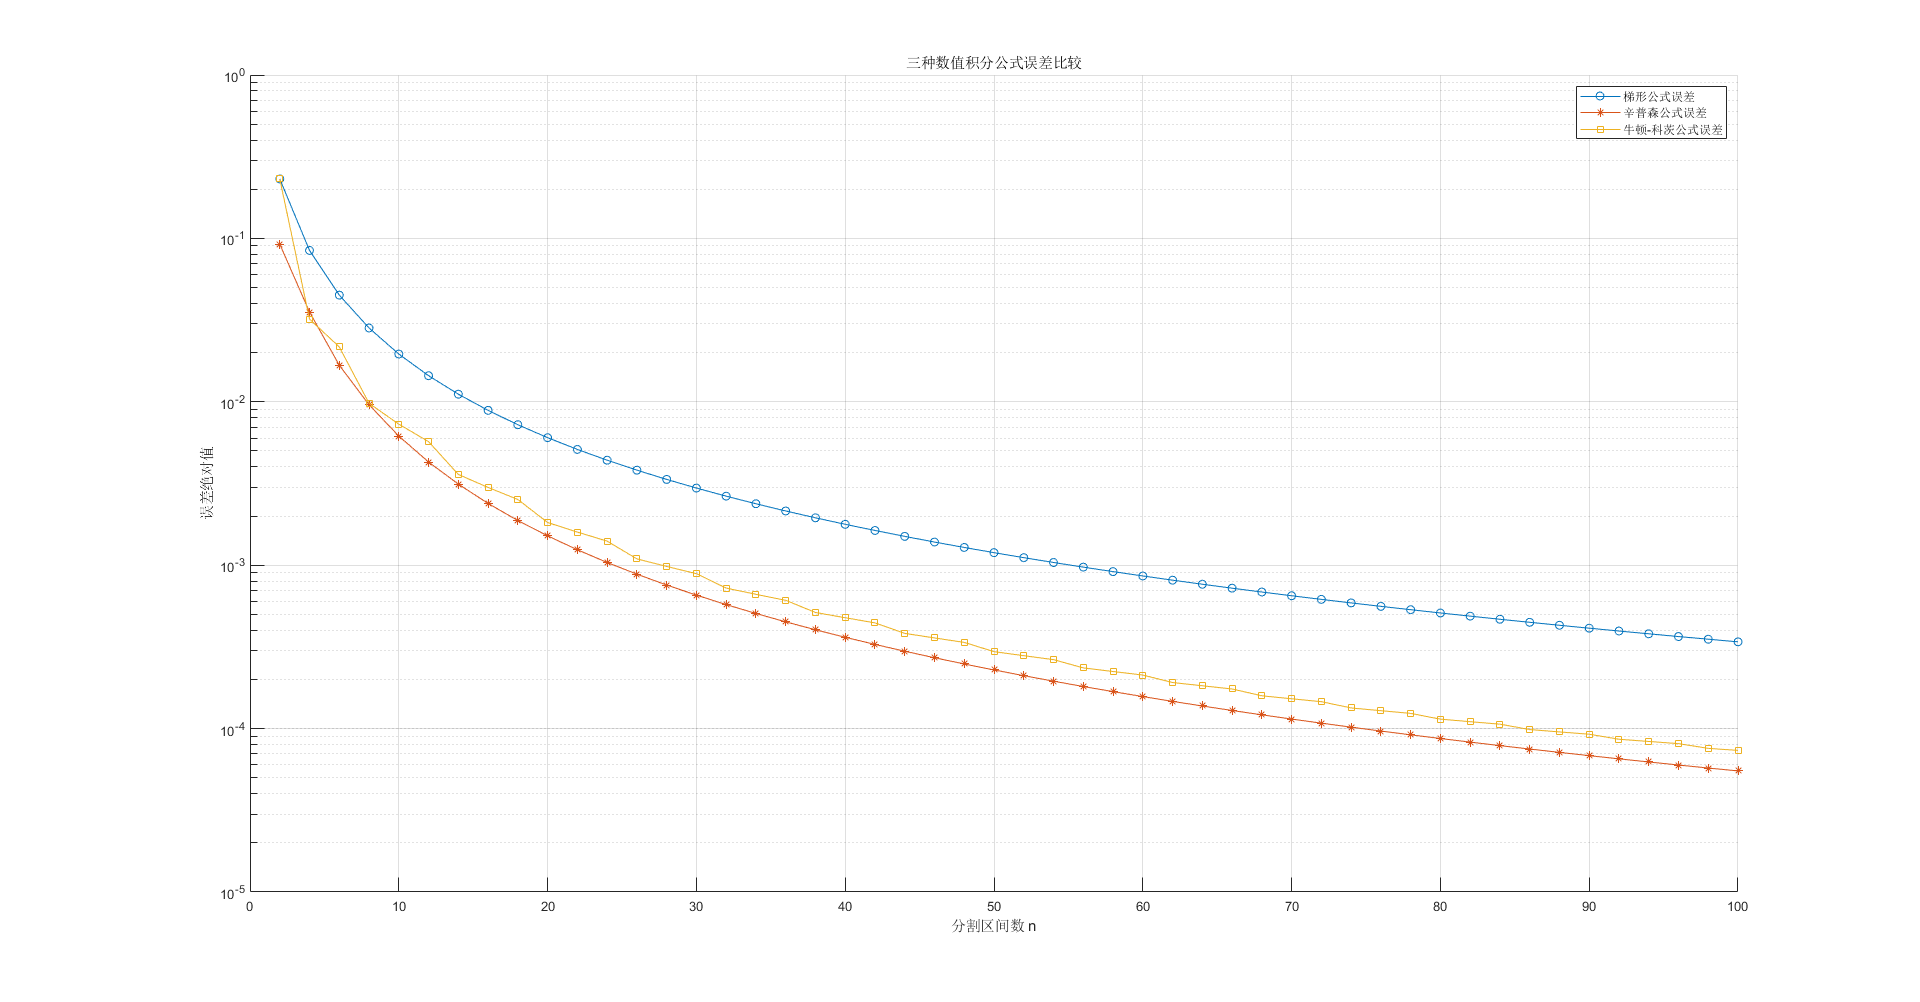
\includegraphics[width=1\linewidth]{figure/4-4-1.png}
    \label{4-4-1}
\end{figure}

\item 高斯-勒让德公式计算正态密度积分

$$
I = \frac{1}{\sqrt{2\pi}} \int_{-1}^1 e^{-x^2/2} dx
$$
\begin{lstlisting}[language=matlab]
f = @(x) 1/sqrt(2*pi) * exp(-x.^2 / 2);

% 2点 Gauss-Legendre（代数精度 3）
x2 = [-1/sqrt(3), 1/sqrt(3)];
w2 = [1, 1];
I_gauss2 = sum(w2 .* f(x2));

% 3点 Gauss-Legendre（代数精度 5）
x3 = [-sqrt(3/5), 0, sqrt(3/5)];
w3 = [5/9, 8/9, 5/9];
I_gauss3 = sum(w3 .* f(x3));

% 精确值（可用 quad 函数估算）
I_true = integral(f, -1, 1, 'AbsTol', 1e-12);

% 显示误差
fprintf('Gauss-2点: %.6f 误差: %.2e\n', I_gauss2, abs(I_gauss2 - I_true));
fprintf('Gauss-3点: %.6f 误差: %.2e\n', I_gauss3, abs(I_gauss3 - I_true));
\end{lstlisting}

\begin{lstlisting}[language=matlab]
Gauss-2点: 0.675395 误差: 7.29e-03
Gauss-3点: 0.682997 误差: 3.08e-04
\end{lstlisting}
\end{enumerate}

\section{实验五}
\subsection*{5.1}
\addcontentsline{toc}{subsection}{5.1}

设 $f(x) = \ln x$，分别取 $h = 1/10^k (k = 1, 2, \ldots, 10)$，用下列 3 个公式分别计算 $f'(0.1)$，$f'(0.3)$，$f'(0.7)$，$f'(1.1)$，$f'(2)$：

\[ f'(x) \approx \frac{f(x+h) - f(x)}{h}, \]
\[ f'(x) \approx \frac{f(x+h) - f(x-h)}{2h}, \]
\[ f'(x) \approx \frac{f(x-2h) - 8f(x-h) + 8f(x+h) - f(x+2h)}{12h}. \]

\begin{enumerate}
    \item 列表比较 3 个公式的计算误差。
    \item 从这里可以得出什么结论？
    \item 再用 Richardson 外推法对上述第 2 个公式的结果进行加速。
\end{enumerate}

Richardson 外推法公式为： $f_j(h)=f_{j-1}(\frac{h}{2})+\frac{f_{j-1}(\frac{h}{2})-f_{j-1}(h)}{4^{j-1}-1}$，取$j=2$即可得两步加速公式。

表中的Inf即表示在此时的条件下部分函数值不存在。

\begin{lstlisting}[language=matlab]
f = @(x) log(x);
f_prime = @(x) 1./x;
xs = [0.1, 0.3, 0.7, 1.1, 2.0];

fprintf('点     h        Forward Error   Central Error   4th-Order Error   Richardson Error\n');
fprintf('--------------------------------------------------------------------------------------\n');

for xi = xs
    for k = 1:10
        h = 1/10^k;

        % 差分近似
        f1 = (f(xi+h) - f(xi)) / h;
        f2 = (f(xi+h) - f(xi-h)) / (2*h);
        f4 = (-f(xi+2*h) + 8*f(xi+h) - 8*f(xi-h) + f(xi-2*h)) / (12*h);

        % Richardson 外推（两步加速）
        f2_next = (f(xi + h/2) - f(xi - h/2)) / h;
        R = (4/3)*f2_next - (1/3)*f2;

        % 真值
        exact = f_prime(xi);

        % 误差
        e1 = abs(f1 - exact);
        e2 = abs(f2 - exact);
        e4 = abs(f4 - exact);
        er = abs(R - exact);

        fprintf('%-5.1f  1e-%-2d   %1.2e     %1.2e     %1.2e      %1.2e\n', xi, k, e1, e2, e4, er);
    end
end
\end{lstlisting}

\begin{lstlisting}[language=matlab]
点     h        Forward Error   Central Error   4th-Order Error   Richardson Error
--------------------------------------------------------------------------------------
0.1    1e-1    3.07e+00     Inf     Inf      Inf
0.1    1e-2    4.69e-01     3.35e-02     8.30e-04      5.05e-05
0.1    1e-3    4.97e-02     3.33e-04     8.00e-08      5.00e-09
0.1    1e-4    5.00e-03     3.33e-06     8.64e-12      0.00e+00
0.1    1e-5    5.00e-04     3.33e-08     0.00e+00      9.70e-12
0.1    1e-6    5.00e-05     2.33e-10     2.91e-11      7.76e-11
0.1    1e-7    5.00e-06     0.00e+00     9.31e-10      4.97e-09
0.1    1e-8    5.07e-07     1.49e-08     1.86e-08      4.47e-08
0.1    1e-9    0.00e+00     2.38e-07     5.96e-08      7.95e-08
0.1    1e-10   3.81e-06     0.00e+00     2.86e-06      0.00e+00
0.3    1e-1    4.57e-01     1.32e-01     5.36e-02      2.28e-03
0.3    1e-2    5.44e-02     1.24e-03     3.31e-06      2.06e-07
0.3    1e-3    5.54e-03     1.23e-05     3.29e-10      2.07e-11
0.3    1e-4    5.55e-04     1.23e-07     6.44e-13      9.10e-13
0.3    1e-5    5.56e-05     1.23e-09     4.85e-12      9.70e-12
0.3    1e-6    5.56e-06     7.76e-11     3.40e-11      2.33e-10
0.3    1e-7    5.54e-07     6.21e-10     1.44e-09      4.35e-09
0.3    1e-8    4.97e-08     2.48e-09     3.10e-09      1.24e-08
0.3    1e-9    1.59e-07     3.97e-08     1.99e-08      1.19e-07
0.3    1e-10   6.36e-07     6.36e-07     3.97e-08      6.36e-07
0.7    1e-1    9.33e-02     9.84e-03     5.13e-04      3.03e-05
0.7    1e-2    1.01e-02     9.72e-05     4.76e-08      2.98e-09
0.7    1e-3    1.02e-03     9.72e-07     4.76e-12      5.05e-13
0.7    1e-4    1.02e-04     9.72e-09     1.30e-13      9.75e-14
0.7    1e-5    1.02e-05     9.20e-11     6.69e-12      1.92e-11
0.7    1e-6    1.02e-06     8.32e-12     4.11e-11      2.25e-10
0.7    1e-7    1.03e-07     8.65e-10     7.48e-10      9.98e-10
0.7    1e-8    3.19e-09     4.26e-09     9.85e-09      5.68e-09
0.7    1e-9    2.55e-08     5.53e-08     5.91e-08      1.43e-07
0.7    1e-10   2.72e-07     2.72e-07     2.13e-07      2.72e-07
1.1    1e-1    3.90e-02     2.52e-03     5.12e-05      3.13e-06
1.1    1e-2    4.11e-03     2.50e-05     4.97e-09      3.11e-10
1.1    1e-3    4.13e-04     2.50e-07     6.16e-13      1.35e-13
1.1    1e-4    4.13e-05     2.50e-09     2.55e-15      2.53e-12
1.1    1e-5    4.13e-06     3.10e-11     9.41e-12      5.54e-12
1.1    1e-6    4.13e-07     6.81e-11     1.09e-10      1.94e-10
1.1    1e-7    4.07e-08     5.50e-10     8.27e-10      2.24e-09
1.1    1e-8    1.02e-08     6.43e-09     9.58e-09      3.95e-09
1.1    1e-9    7.18e-08     7.18e-08     1.14e-07      7.18e-08
1.1    1e-10   8.67e-08     2.71e-08     7.18e-08      1.07e-07
2.0    1e-1    1.21e-02     4.17e-04     2.52e-06      1.57e-07
2.0    1e-2    1.25e-03     4.17e-06     2.50e-10      1.56e-11
2.0    1e-3    1.25e-04     4.17e-08     9.24e-14      1.89e-14
2.0    1e-4    1.25e-05     4.17e-10     6.82e-13      1.97e-12
2.0    1e-5    1.25e-06     7.28e-12     8.19e-12      2.43e-12
2.0    1e-6    1.25e-07     0.00e+00     2.91e-11      1.55e-10
2.0    1e-7    1.30e-08     4.66e-10     3.49e-10      1.55e-10
2.0    1e-8    0.00e+00     0.00e+00     4.66e-09      0.00e+00
2.0    1e-9    0.00e+00     0.00e+00     5.22e-08      0.00e+00
2.0    1e-10   0.00e+00     0.00e+00     3.58e-07      0.00e+00
\end{lstlisting}

结论：总体上Richardson Error减小最快，其次4th-Order Error，之后是Central Error，最后是Forward Erro，收敛速度也与我们所学的基本一致。另外，h减小大多数但并不总意味着公式更精确，数据中有大量例子证明了这一点，此外，当误差减小到一定程度时，计算方法的规律变得不明显。另外注意到，为了避免两个过小的数相减，应当先在计算中除以$h$。

\subsection*{5.2}
\addcontentsline{toc}{subsection}{5.2}
设 $f(x) = \sin(5x^2 - 21)$.

\begin{enumerate}
    \item 分别利用前差公式和后差公式计算 $f'(0.79)$ 的近似值和误差，取 4 位小数点计算，其中步长分别取 $h = 0.1, 0.01, 0.001, 0.0001$，$|f'(x)| \leq 80, x \in [0, 1]$.
    \item 将 (1) 中计算的 $f'(0.79)$ 的近似值分别与精确值比较。
\end{enumerate}

使用前向差分公式：
    $$
    f'(x) \approx \frac{f(x + h) - f(x)}{h}
    $$
    
后向差分公式：
    $$
    f'(x) \approx \frac{f(x) - f(x - h)}{h}
    $$
    
点：$x = 0.79$，步长 $h = 0.1, 0.01, 0.001, 0.0001$

精确导数为：

  $$
  f'(x) = \cos(5x^2 - 21) \cdot 10x
  $$

\begin{lstlisting}[language=matlab]
% 定义函数及其导数
f = @(x) sin(5*x.^2 - 21);
f_prime = @(x) cos(5*x.^2 - 21) .* 10 .* x;

x0 = 0.79;
hs = [0.1, 0.01, 0.001, 0.0001];
true_val = f_prime(x0); % 精确值

fprintf('h        前向差值     误差        后向差值     误差\n');
fprintf('------------------------------------------------------\n');

for h = hs
    % 前向差分
    f_forward = (f(x0 + h) - f(x0)) / h;

    % 后向差分
    f_backward = (f(x0) - f(x0 - h)) / h;

    % 误差
    err_forward = abs(f_forward - true_val);
    err_backward = abs(f_backward - true_val);

    fprintf('%.4f   %.4f  %.2e   %.4f  %.2e\n', ...
        h, f_forward, err_forward, f_backward, err_backward);
end
\end{lstlisting}

\begin{lstlisting}[language=matlab]
h        前向差值     误差        后向差值     误差
------------------------------------------------------
0.1000   1.4660  3.00e+00   5.9689  1.50e+00
0.0100   4.2285  2.37e-01   4.6867  2.21e-01
0.0010   4.4425  2.30e-02   4.4883  2.28e-02
0.0001   4.4632  2.29e-03   4.4678  2.29e-03
\end{lstlisting}


\subsection*{5.3}
\addcontentsline{toc}{subsection}{5.3}

设已给出 $y = f(x)$ 的数据表如下：

\begin{table}[h]
\centering
\caption{函数 $f(x)$ 的数据表}
\label{tab:data}
\begin{tabular}{c|ccccccc}
\toprule
$x$       & 1.0000 & 1.1000 & 1.2000 & 1.3000 & 1.4000 & 1.5000 & 1.6000 \\
\midrule
$f(x)$    & 0.2500 & 0.2268 & 0.2066 & 0.1890 & 0.1736 & 0.1600 & 0.1479 \\
\bottomrule
\end{tabular}
\end{table}

已知 $M = 0.7502$，试用三点公式计算下列问题：

\begin{enumerate}
    \item 当 $h=0.1$ 时，计算 $y = f(x)$ 在 $x=1.0000$, $1.1000$, $1.2000$, $1.3000$, $1.4000$, $1.5000$, $1.6000$ 处的一阶导数的近似值，并估计误差。
    \item 当 $h=0.2$ 时，计算 $y = f(x)$ 在 $x=1.0000$, $1.2000$, $1.4000$, $1.6000$ 处的一阶导数的近似值，并估计误差。
    \item 当 $h=0.3$ 时，计算 $y = f(x)$ 在 $x=1.0000$, $1.3000$, $1.6000$ 处的一阶导数的近似值，并估计误差。
    \item 表\ref{tab:data}中的数据是函数 $f(x) = \frac{1}{(1+x)^2}$ 在相应点的数值，将1至3计算的一阶导数的近似值与精确值 $f'(x) = -\frac{2}{(1+x)^3}$ 比较，并求出它们的绝对误差。
\end{enumerate}

$$
f(x) = \frac{1}{(1 + x)^2}, \quad \text{则导数为} \quad f'(x) = \frac{-2}{(1 + x)^3}
$$

\begin{table}[ht]
\centering
\caption{一阶导数三点差分公式}
\label{5-3-1}
\begin{tabular}{c|c|c|c}
\toprule
位置 & 差分公式 & 适用范围 & 误差阶 \\
\midrule
向前差分（前端点） & 
$\displaystyle f'(x_i) \approx \frac{-3f_i + 4f_{i+1} - f_{i+2}}{2h}$ & 
区间起始点 $i=1$ & $O(h^2)$ \\
\midrule
中心差分（中间点） & 
$\displaystyle f'(x_i) \approx \frac{f_{i+1} - f_{i-1}}{2h}$ & 
区间内部点 $1 < i < n$ & $O(h^2)$ \\
\midrule
向后差分（末端点） & 
$\displaystyle f'(x_i) \approx \frac{f_{i-2} - 4f_{i-1} + 3f_i}{2h}$ & 
区间末端点 $i=n$ & $O(h^2)$ \\
\bottomrule
\end{tabular}
\end{table}

\begin{lstlisting}[language=matlab]
clc; clear;

% 原始数据
x_all = 1.0:0.1:1.6;
f_all = [0.2500, 0.2268, 0.2066, 0.1890, 0.1736, 0.1600, 0.1479];

% 精确导函数
f_prime = @(x) -2 ./ (1 + x).^3;

%% h = 0.1
h1 = 0.1;
df_h01 = zeros(1, 7);

% 前向差分
df_h01(1) = (-3*f_all(1) + 4*f_all(2) - f_all(3)) / (2*h1);
% 中心差分
for i = 2:6
    df_h01(i) = (f_all(i+1) - f_all(i-1)) / (2*h1);
end
% 后向差分
df_h01(7) = (f_all(5) - 4*f_all(6) + 3*f_all(7)) / (2*h1);

x_h01 = x_all;
true_h01 = f_prime(x_h01);
error_h01 = abs(df_h01 - true_h01);

%% h = 0.2
h2 = 0.2;
df_h02 = zeros(1, 4);
% 对应点索引：1,3,5,7
df_h02(1) = (-3*f_all(1) + 4*f_all(2) - f_all(3)) / (2*h2);    % forward
df_h02(2) = (f_all(4) - f_all(2)) / (2*h2);                   % center
df_h02(3) = (f_all(6) - f_all(4)) / (2*h2);                   % center
df_h02(4) = (f_all(5) - 4*f_all(6) + 3*f_all(7)) / (2*h2);    % backward

x_h02 = [1.0, 1.2, 1.4, 1.6];
true_h02 = f_prime(x_h02);
error_h02 = abs(df_h02 - true_h02);

%% h = 0.3
h3 = 0.3;
df_h03 = zeros(1, 3);
% 对应点：1.0, 1.3, 1.6 => 索引 1,4,7
df_h03(1) = (-3*f_all(1) + 4*f_all(3) - f_all(5)) / (2*h3);    % forward
df_h03(2) = (f_all(5) - f_all(1)) / (2*h3);                    % center
df_h03(3) = (f_all(3) - 4*f_all(5) + 3*f_all(7)) / (2*h3);     % backward

x_h03 = [1.0, 1.3, 1.6];
true_h03 = f_prime(x_h03);
error_h03 = abs(df_h03 - true_h03);

%% 打印结果
fprintf('h = 0.1:\n   x       Approx        Exact         Abs.Error\n');
for i = 1:length(x_h01)
    fprintf('%.1f   %.6f   %.6f   %.2e\n', x_h01(i), df_h01(i), true_h01(i), error_h01(i));
end

fprintf('\nh = 0.2:\n   x       Approx        Exact         Abs.Error\n');
for i = 1:length(x_h02)
    fprintf('%.1f   %.6f   %.6f   %.2e\n', x_h02(i), df_h02(i), true_h02(i), error_h02(i));
end

fprintf('\nh = 0.3:\n   x       Approx        Exact         Abs.Error\n');
for i = 1:length(x_h03)
    fprintf('%.1f   %.6f   %.6f   %.2e\n', x_h03(i), df_h03(i), true_h03(i), error_h03(i));
end
\end{lstlisting}

\begin{lstlisting}[language=matlab]
h = 0.1:
   x       Approx        Exact         Abs.Error
1.0   -0.247000   -0.250000   3.00e-03
1.1   -0.217000   -0.215959   1.04e-03
1.2   -0.189000   -0.187829   1.17e-03
1.3   -0.165000   -0.164379   6.21e-04
1.4   -0.145000   -0.144676   3.24e-04
1.5   -0.128500   -0.128000   5.00e-04
1.6   -0.113500   -0.113792   2.92e-04

h = 0.2:
   x       Approx        Exact         Abs.Error
1.0   -0.123500   -0.250000   1.27e-01
1.2   -0.094500   -0.187829   9.33e-02
1.4   -0.072500   -0.144676   7.22e-02
1.6   -0.056750   -0.113792   5.70e-02

h = 0.3:
   x       Approx        Exact         Abs.Error
1.0   -0.162000   -0.250000   8.80e-02
1.3   -0.127333   -0.164379   3.70e-02
1.6   -0.073500   -0.113792   4.03e-02
\end{lstlisting}


\section{实验六}
\subsection*{6.1}
\addcontentsline{toc}{subsection}{6.1}
给定初值问题

$y' = \frac{2}{t}y + t^2 e^t, \quad 1 \leq t \leq 2, \quad y(1) = 0,$

其精确解为 $y(t) = t^2(e^t - e)$：

(1) 取 $h = 0.1$，用 4 阶 Runge-Kutta 方法求上述初值问题的近似解，并将它们与 y 的实际值进行比较；

(2) 用(1)中所得的答案分别用分段线性插值、分段三次 Hermite 插值、三次样条求在下列值处的近似 y，并将它们与 y 的实际值进行比较。
(i) $y(1.04)$, (ii) $y(1.55)$, (iii) $y(1.97)$

\begin{lstlisting}[language=matlab]
% 定义微分方程及精确解
f = @(t, y) (2./t).*y + t.^2 .* exp(t);
y_exact = @(t) t.^2 .* (exp(t) - exp(1));

% 初值与步长
t0 = 1; y0 = 0; h = 0.1;
t = t0:h:2;
n = length(t);
y = zeros(1, n);
y(1) = y0;

% RK4 方法求解 ODE
for i = 1:n-1
    k1 = h * f(t(i), y(i));
    k2 = h * f(t(i) + h/2, y(i) + k1/2);
    k3 = h * f(t(i) + h/2, y(i) + k2/2);
    k4 = h * f(t(i) + h, y(i) + k3);
    y(i+1) = y(i) + (k1 + 2*k2 + 2*k3 + k4)/6;
end

% 输出比较
fprintf('   t       RK4 Approx     Exact        Error\n');
for i = 1:n
    exact_val = y_exact(t(i));
    fprintf('%.2f     %.6f    %.6f    %.2e\n', t(i), y(i), exact_val, abs(y(i) - exact_val));
end

% 查询点
query_points = [1.04, 1.55, 1.97];
true_vals = y_exact(query_points);

% ----------------------------
% 插值方法

% 1. 分段线性插值
linear_vals = interp1(t, y, query_points, 'linear');

% 2. 分段三次 Hermite 插值（makima 近似）
hermite_vals = interp1(t, y, query_points, 'makima');

% 3. 三次样条插值（默认自然边界条件）
spline_vals = interp1(t, y, query_points, 'spline');

% ----------------------------
% 打印结果比较
fprintf('  x     Exact       Linear      Hermite     Spline\n');
for i = 1:length(query_points)
    fprintf('%.2f  %.6f  %.6f  %.6f  %.6f\n', ...
        query_points(i), ...
        true_vals(i), ...
        linear_vals(i), ...
        hermite_vals(i), ...
        spline_vals(i));
end
\end{lstlisting}

\begin{lstlisting}[language=matlab]
1.00     0.000000    0.000000    0.00e+00
1.10     0.345910    0.345920    9.59e-06
1.20     0.866622    0.866643    2.08e-05
1.30     1.607181    1.607215    3.37e-05
1.40     2.620311    2.620360    4.82e-05
1.50     3.967602    3.967666    6.44e-05
1.60     5.720879    5.720962    8.22e-05
1.70     7.963772    7.963873    1.02e-04
1.80     10.793502    10.793625    1.23e-04
1.90     14.322936    14.323082    1.46e-04
2.00     18.682927    18.683097    1.71e-04
  x     Exact       Linear      Hermite     Spline
1.04  0.119987  0.138364  0.115037  0.120170
1.55  4.788635  4.844241  4.789124  4.788532
1.97  17.279298  17.374929  17.292003  17.279703
\end{lstlisting}

\subsection*{6.2}
\addcontentsline{toc}{subsection}{6.2}
地球卫星的轨道是一个椭圆，椭圆的周长计算公式为：

\[ s = a \int_0^{\pi/2} \sqrt{1 - (c/a)^2 \sin \theta} \, \mathrm{d}\theta \]

其中，$a$ 为椭圆长半轴，$c$ 为椭圆中心与地球中心的距离，令 $H, h$ 分别为远地点、近地点的距离，$R=6371$ 千米为地球半径，则 $a = (2R + h + H)/2, c = (H - h)/2$，其中我国第一颗人造卫星 $H = 3484$ 千米，$h = 439$ 千米。

分别通过复化梯形公式、Romberg 积分、复化 Simpson 公式计算卫星轨道的周长，研究并比较这三种算法的收敛性。


\begin{enumerate}
    \item 复化梯形公式（Composite Trapezoidal Rule）：
    
    将区间 $[a,b]$ 等分成 $n$ 个子区间，步长 $h = \frac{b - a}{n}$，节点为 $x_0 = a, x_1 = a + h, \dots, x_n = b$。

    复化梯形公式为：
    
    $$
    \int_a^b f(x)\, dx \approx \frac{h}{2} \left[ f(x_0) + 2 \sum_{i=1}^{n-1} f(x_i) + f(x_n) \right]
    $$

    \item Romberg 积分（Romberg Integration）：
    
    设 $T_{m,1}$ 是用步长 $h_m = \frac{b-a}{2^{m-1}}$ 的复化梯形公式结果：

    $$
    T_{m,1} = \text{复化梯形公式},\quad m = 1, 2, \dots
    $$

    然后用递推公式计算高阶逼近：
    
    $$
    T_{m,k} = \frac{4^{k-1} T_{m,k-1} - T_{m-1,k-1}}{4^{k-1} - 1}, \quad k = 2,3,\dots,m
    $$

    最终结果是 $T_{m,m}$，即误差阶为 $O(h^{2m})$ 的高精度近似。
    \item 复化 Simpson 公式（Composite Simpson's Rule）
    将区间 $[a,b]$ 等分成 偶数个子区间，设 $n$ 为偶数，步长 $h = \frac{b - a}{n}$，节点为 $x_0, x_1, \dots, x_n$。

    复化 Simpson 公式为：
    
    $$
    \int_a^b f(x)\, dx \approx \frac{h}{3} \left[ f(x_0) + 4 \sum_{\text{奇数 } i=1}^{n-1} f(x_i) + 2 \sum_{\text{偶数 } i=2}^{n-2} f(x_i) + f(x_n) \right]
    $$
\end{enumerate}

\begin{lstlisting}[language=matlab]
clc; clear;
% 地球半径与卫星参数
R = 6371;
H = 3484;
h = 439;

a = (2 * R + H + h) / 2;
c = (H - h) / 2;
e2 = (c / a)^2;

% 被积函数
f = @(theta) sqrt(1 - e2 * sin(theta));

% 高精度参考值
s_ref = a * integral(f, 0, pi/2, 'AbsTol', 1e-12);

% 自定义复化梯形
composite_trap = @(f, a_, b_, n) ...
    (b_ - a_) / n * (0.5*f(a_) + sum(f(a_ + (1:n-1)*(b_ - a_)/n)) + 0.5*f(b_));

% 自定义复化 Simpson
composite_simp = @(f, a_, b_, n) ...
    ((b_ - a_) / (3*n)) * (f(a_) + ...
    4 * sum(f(a_ + (1:2:n-1)*(b_ - a_)/n)) + ...
    2 * sum(f(a_ + (2:2:n-2)*(b_ - a_)/n)) + f(b_));

% 自定义 Romberg 积分（生成 Romberg 表，返回 T(m,m)）
romberg_integrate = @(f, a_, b_, m) ...
    romberg_core(f, a_, b_, m);

% 精度比较
N = 2.^(1:10);
trap_error = zeros(size(N));
simp_error = zeros(size(N));
romb_error = zeros(size(N));

for i = 1:length(N)
    n = N(i);
    % 复化梯形
    s_trap = a * composite_trap(f, 0, pi/2, n);
    trap_error(i) = abs(s_trap - s_ref);

    % Simpson（n 必须为偶数）
    n_simp = n; if mod(n_simp, 2) ~= 0, n_simp = n_simp + 1; end
    s_simp = a * composite_simp(f, 0, pi/2, n_simp);
    simp_error(i) = abs(s_simp - s_ref);

    % Romberg（m = i）
    s_romb = a * romberg_integrate(f, 0, pi/2, i);  % 使用 i 层
    romb_error(i) = abs(s_romb - s_ref);
end

% 最终结果输出
s_trap_final = a * composite_trap(f, 0, pi/2, 1024);
s_simp_final = a * composite_simp(f, 0, pi/2, 1024);
s_romb_final = a * romberg_integrate(f, 0, pi/2, 10);

fprintf('高精度参考值: %.12f\n', s_ref);
fprintf('复化梯形结果: %.12f\n', s_trap_final);
fprintf('复化Simpson结果: %.12f\n', s_simp_final);
fprintf('Romberg结果    : %.12f\n', s_romb_final);

% 绘图
loglog(N, trap_error, 'o-', 'DisplayName', 'Trapezoidal Error'); hold on;
loglog(N, simp_error, 's-', 'DisplayName', 'Simpson Error');
loglog(N, romb_error, 'd-', 'DisplayName', 'Romberg Error');
xlabel('n = 2^k (子区间数)');
ylabel('误差');
legend('Location', 'southwest');
title('复化梯形 / Simpson / Romberg误差对比');
grid on;

function I = romberg_core(f, a, b, m)
    R = zeros(m, m);
    for k = 1:m
        n = 2^(k-1);
        h = (b - a)/n;
        x = linspace(a, b, n+1);
        R(k,1) = h * (0.5*f(a) + sum(f(x(2:end-1))) + 0.5*f(b));  % T_{k,1}
    end

    for j = 2:m
        for k = j:m
            R(k,j) = (4^(j-1)*R(k,j-1) - R(k-1,j-1)) / (4^(j-1) - 1);
        end
    end

    I = R(m,m);
end
\end{lstlisting}

\begin{lstlisting}[language=matlab]
高精度参考值: 12948.641137983348
复化梯形结果: 12948.641165258541
复化Simpson结果: 12948.641137983344
Romberg结果    : 12948.641137983346
\end{lstlisting}

\begin{figure}
    \centering
    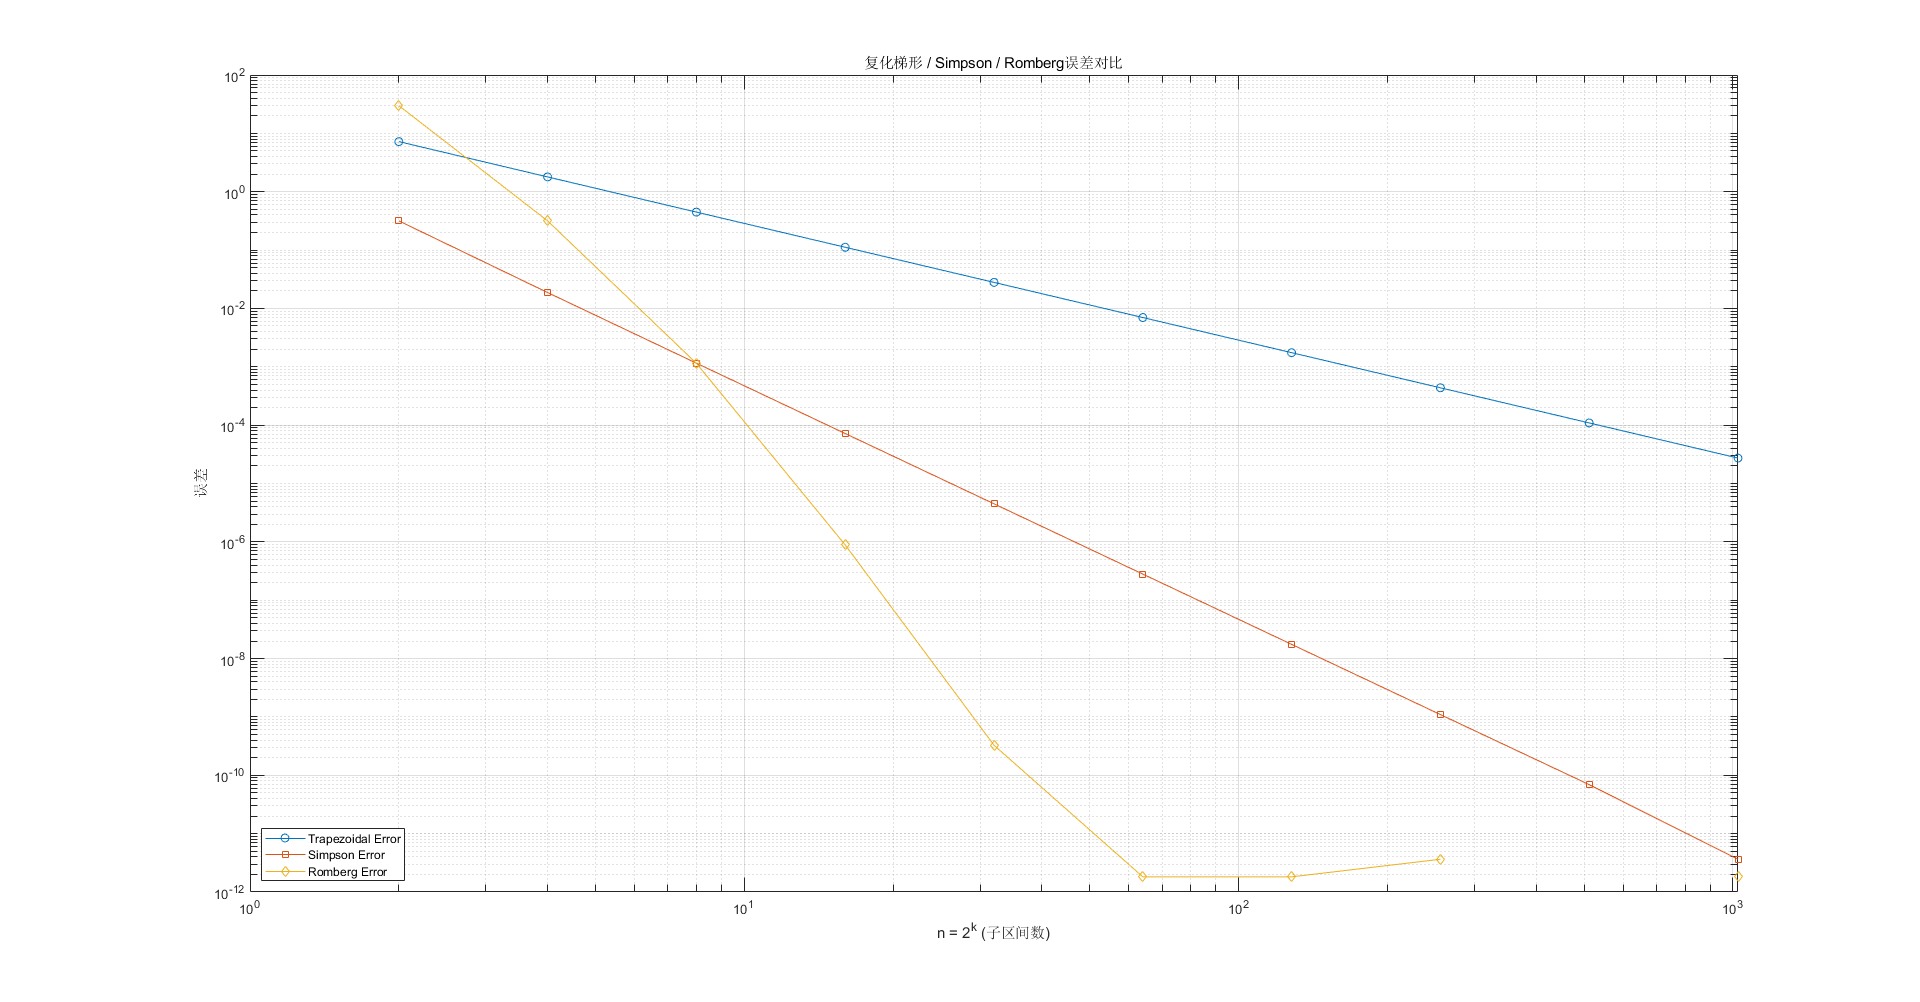
\includegraphics[width=1\linewidth]{figure/6-2-1.png}
    \label{6-2-1}
\end{figure}

Romberg算法收敛最快，复化Simpson齐次，复化梯形再次。三者的计算精度基本都随区间数量的增多而增大，但区间数量增大到一定程度时，变化不再明显。

\subsection*{6.4}
\addcontentsline{toc}{subsection}{6.4}
一敌舰在某海域内沿正北方向航行时，我方战舰恰位于敌舰的正西方 1 海里处。我舰向敌舰发射鱼雷，敌舰速度为 0.42 海里/分，鱼雷速度为敌舰速度的两倍。试问敌舰航行多远时将被击中？

提示：本问题归结为常微分方程初值问题

直接通过龙格库塔方法进行数值模拟即可。

\[
\begin{cases}
y'' = \frac{\sqrt{1 + y'^2}}{2(1 - x)}, & x \in (0, 1), \\
y|_{x=0} = 0, & y'|_{x=0} = 0.
\end{cases}
\]


\begin{lstlisting}[language=matlab]
clc; clear;

% 定义微分方程组
% y1 = y, y2 = y'
f = @(x, Y) [Y(2);
             sqrt(1 + Y(2)^2) / (2 * (1 - x))];

% 初始条件
x0 = 0;
y0 = [0; 0];  % y(0) = 0, y'(0) = 0

% 积分区间与步长
h = 1e-3;
x = x0:h:0.999;  % 避免除以0
n = length(x);

% 初始化解
Y = zeros(2, n);
Y(:,1) = y0;

% 4阶 Runge-Kutta 求解
for i = 1:n-1
    k1 = f(x(i), Y(:,i));
    k2 = f(x(i) + h/2, Y(:,i) + h/2 * k1);
    k3 = f(x(i) + h/2, Y(:,i) + h/2 * k2);
    k4 = f(x(i) + h,   Y(:,i) + h * k3);
    Y(:,i+1) = Y(:,i) + h/6 * (k1 + 2*k2 + 2*k3 + k4);
end

% 最后一个 y 值即为敌舰被击中时航行的距离
fprintf('敌舰航行的距离约为 %.6f 海里\n', Y(1,end));

% 绘图
plot(x, Y(1,:), 'b', 'LineWidth', 2);
xlabel('x（鱼雷水平位移）');
ylabel('y（鱼雷垂直位移 / 敌舰航行距离）');
title('鱼雷轨迹 y(x)');
grid on;
\end{lstlisting}

\begin{lstlisting}[language=matlab]
敌舰航行的距离约为 0.635037 海里
\end{lstlisting}
\begin{figure}
    \centering
    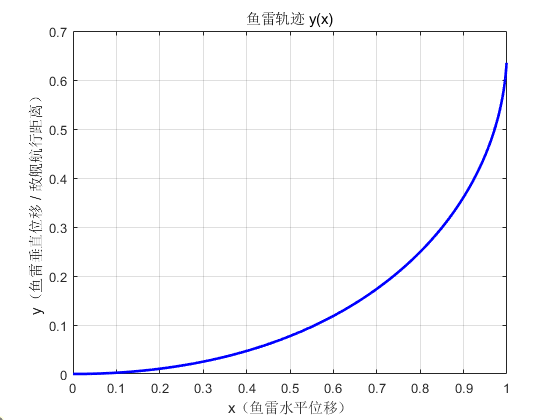
\includegraphics[width=1\linewidth]{figure/6-4-1.png}
    \label{6-4-1}
\end{figure}

\section{实验七}
\subsection*{7.3}
\addcontentsline{toc}{subsection}{7.3}
基于插值法的超分辨图像重建

对于一幅图像可以将其定义为一个二维函数：$H(x, y)$，其中 $x$ 和 $y$ 是空间坐标，在 $x-y$ 平面中任何一对空间坐标$(x, y)$上的幅值 $H$ 称为该点图像的强度、亮度或灰度。当 $x, y$ 和幅值 $f$ 为有限的、离散的数值时，称该图像为数字图像。注意，数字图像是由有限数量的元素组成的。每个元素都有一个特殊的位置和数值。这些元素称为图片元素。图像元素和像素。像素是用来定义图像元素最广泛的术语。低分辨率图像在成像的过程中受到很多退化因素的影响，运动变换、成像模糊和降采样是其中最主要的三个因素。整个过程可以通过使下面的线性变换模型来表征。

\[ L = DBFH + N \]

式中，$L$ 表示观测图像所对应的矩阵，$H$ 表示输入的高分辨率图像，$F$ 表示运动变换矩阵，通常由运动、平移等因素造成，$B$ 表示模糊作用矩阵，通常由环境或成像系统本身引起，$D$ 表示采样矩阵，通常由成像系统的分辨率决定，$N$ 表示加性噪声，通常来自于成像环境或成像过程。选取一幅图像，完成以下工作：
(1) 下采样：通过删除图像的偶数行和偶数列将图像放缩为原图的 $1/2$；
(2) 上采样：通过最近邻、双线性以及双三次插值三种方法对图像进行重建；
(3) 给出运行时间对比以及客观评价结果。


\verb|matlab|为我们提供了丰富的图像处理工具，我们只需要调用即可完成任务。关于客观评价结果，可以采用PSNR（Peak Signal-to-Noise Ratio，峰值信噪比），它是一种广泛用于衡量图像/视频质量的客观指标。
\begin{lstlisting}[language=matlab]
clc; clear; close all;
I = imread('peppers.png');  % 示例彩色图
if size(I,3) == 3
    I = rgb2gray(I); % 转为灰度
end
I = im2double(I);

% 原图大小
[H, W] = size(I);

% 1. 下采样：删除偶数行和偶数列
I_down = I(1:2:end, 1:2:end);

% 显示原图和下采样图像
figure; 
subplot(2,3,1); imshow(I); title('原图');
subplot(2,3,2); imshow(I_down); title('下采样(1/2)');

% 2. 上采样恢复，目标恢复至原图大小(H x W)
scale = 2;

% 最近邻插值
tic;
I_nn = imresize(I_down, [H, W], 'nearest');
time_nn = toc;

% 双线性插值
tic;
I_bilinear = imresize(I_down, [H, W], 'bilinear');
time_bilinear = toc;

% 双三次插值
tic;
I_bicubic = imresize(I_down, [H, W], 'bicubic');
time_bicubic = toc;

% 显示重建图像
subplot(2,3,3); imshow(I_nn); title(sprintf('最近邻插值 (%.4fs)', time_nn));
subplot(2,3,4); imshow(I_bilinear); title(sprintf('双线性插值 (%.4fs)', time_bilinear));
subplot(2,3,5); imshow(I_bicubic); title(sprintf('双三次插值 (%.4fs)', time_bicubic));

% 3. 客观评价：计算PSNR
psnr_nn = psnr(I_nn, I);
psnr_bilinear = psnr(I_bilinear, I);
psnr_bicubic = psnr(I_bicubic, I);

% 输出评价结果
fprintf('插值方法\t运行时间(s)\tPSNR(dB)\n');
fprintf('最近邻插值\t%.4f\t\t%.4f\n', time_nn, psnr_nn);
fprintf('双线性插值\t%.4f\t\t%.4f\n', time_bilinear, psnr_bilinear);
fprintf('双三次插值\t%.4f\t\t%.4f\n', time_bicubic, psnr_bicubic);
\end{lstlisting}

\begin{lstlisting}[language=matlab]
插值方法	运行时间(s)	PSNR(dB)
最近邻插值	0.0024		31.3079
双线性插值	0.0014		33.4334
双三次插值	0.0010		33.4069
\end{lstlisting}

\begin{figure}
    \centering
    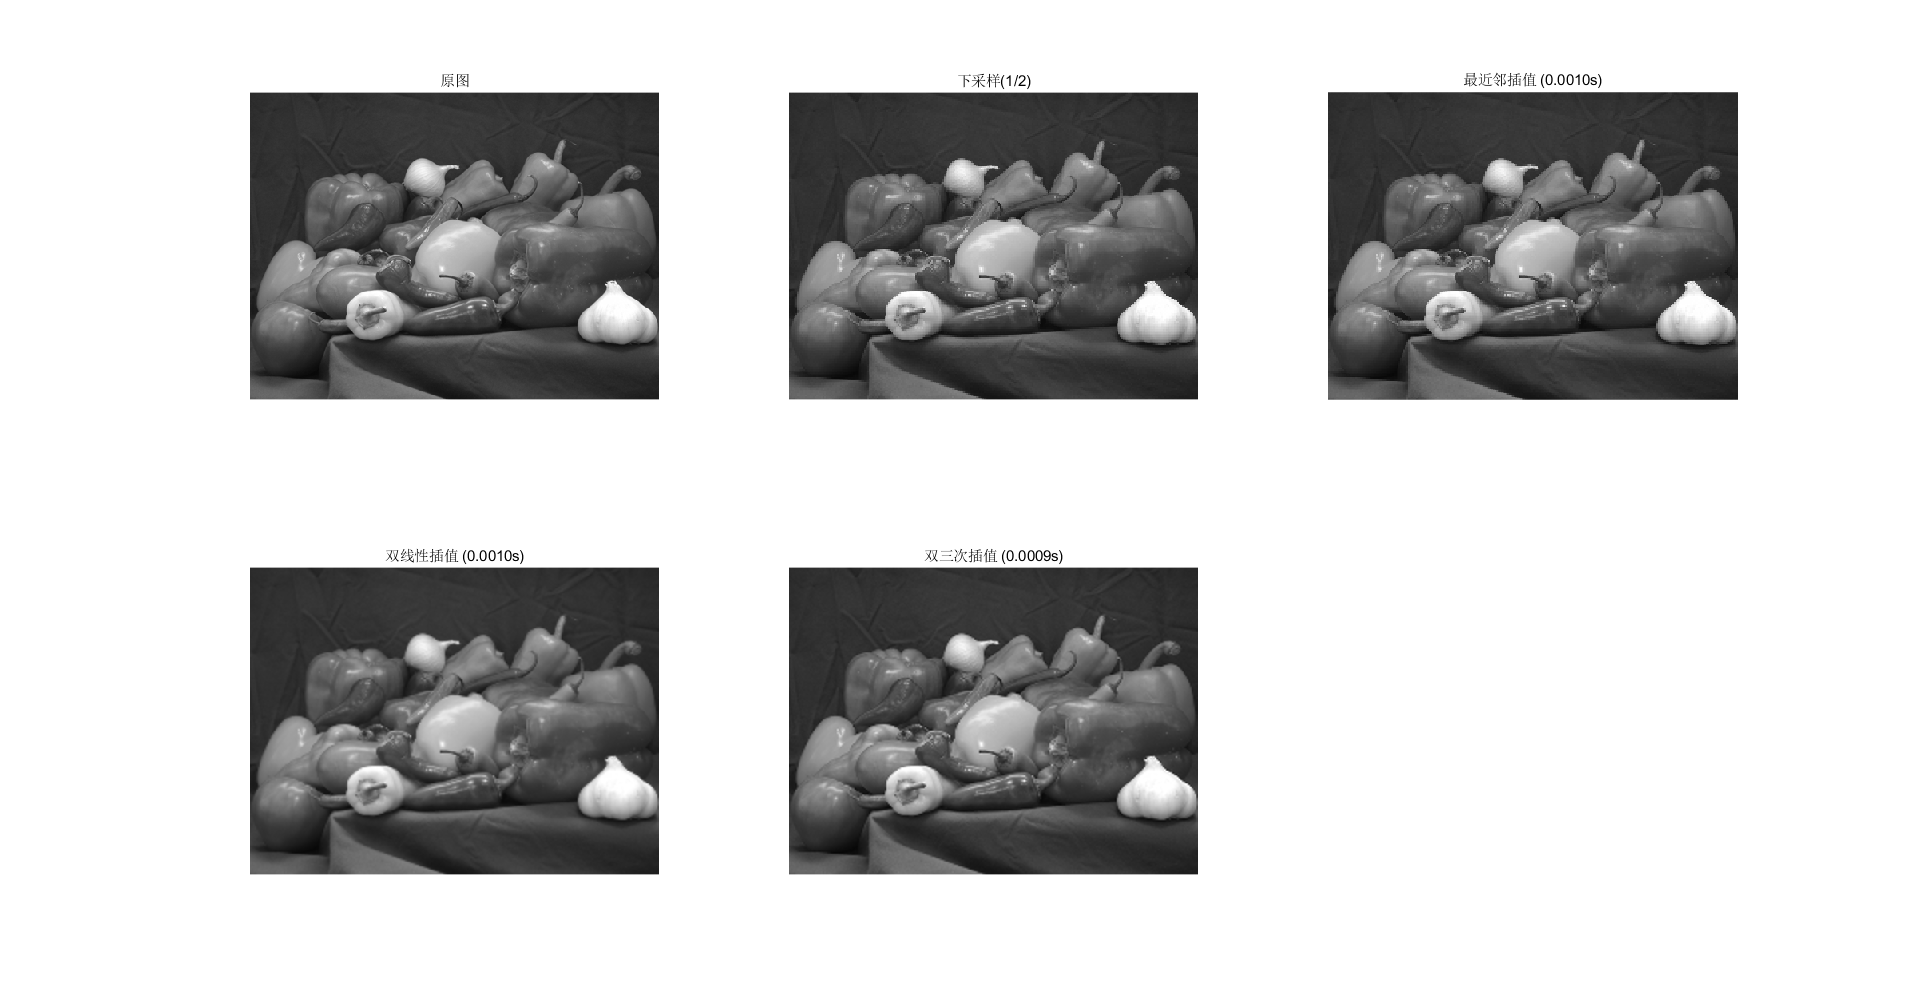
\includegraphics[width=1\linewidth]{figure/7-3-1.png}
    \label{7-3-1}
\end{figure}

\subsection*{7.5}
\addcontentsline{toc}{subsection}{7.5}
数值微分

设 $\mathbf{X \in R^{m \times n}}$ 表示未知的真实图像所对应的矩阵，$\mathbf{Y \in R^{m \times n}}$ 表示观测到的噪声图像，全变分模型表示为：

\[ \hat{X} = \arg \min_{X} \|Y - X\|_F^2 + \lambda \|X\|_{TV} \]

这里 Frobenius 范数 \(\|\| \cdot \|_F\) 保证图像 Y 与图像 X 的所有元素的平方和足够小，\(\|X\|_{TV} = \sum_{i,j} |X_{i,j}\) 表示图像对应的水平方向梯度与数值方向梯度值的绝对值之和，\(\lambda\) 是平衡正则项与数据保真项关系的因子。

(1) 选取近照一张，对图像添加噪声方差为 20 的高斯白噪声，并计算噪声图像 Y 与真实图像 X 的水平梯度图像以及竖直梯度图像；

(2) 求解全变分模型，利用 TV loss 对噪声图像去噪，并计算噪声图像与去噪图像的 PSNR 和 SSIM 数值。

\begin{lstlisting}[language=matlab]
clc; clear;

% 读取灰度图像
X = im2double(imread('cameraman.tif'));  % 大小为 m×n
[m, n] = size(X);

% 添加方差为 20 的高斯白噪声
sigma = sqrt(20)/255;
Y = imnoise(X, 'gaussian', 0, sigma^2);

% 计算水平与竖直梯度（中心差分或向前差分）
Gx = Y(:, [2:end end]) - Y;    % 水平梯度（向右差分）
Gy = Y([2:end end], :) - Y;    % 竖直梯度（向下差分）

% 显示结果
figure;
subplot(2,2,1); imshow(X); title('Original Image X');
subplot(2,2,2); imshow(Y); title('Noisy Image Y');
subplot(2,2,3); imshow(Gx, []); title('Horizontal Gradient');
subplot(2,2,4); imshow(Gy, []); title('Vertical Gradient');
\end{lstlisting}
\begin{figure}
    \centering
    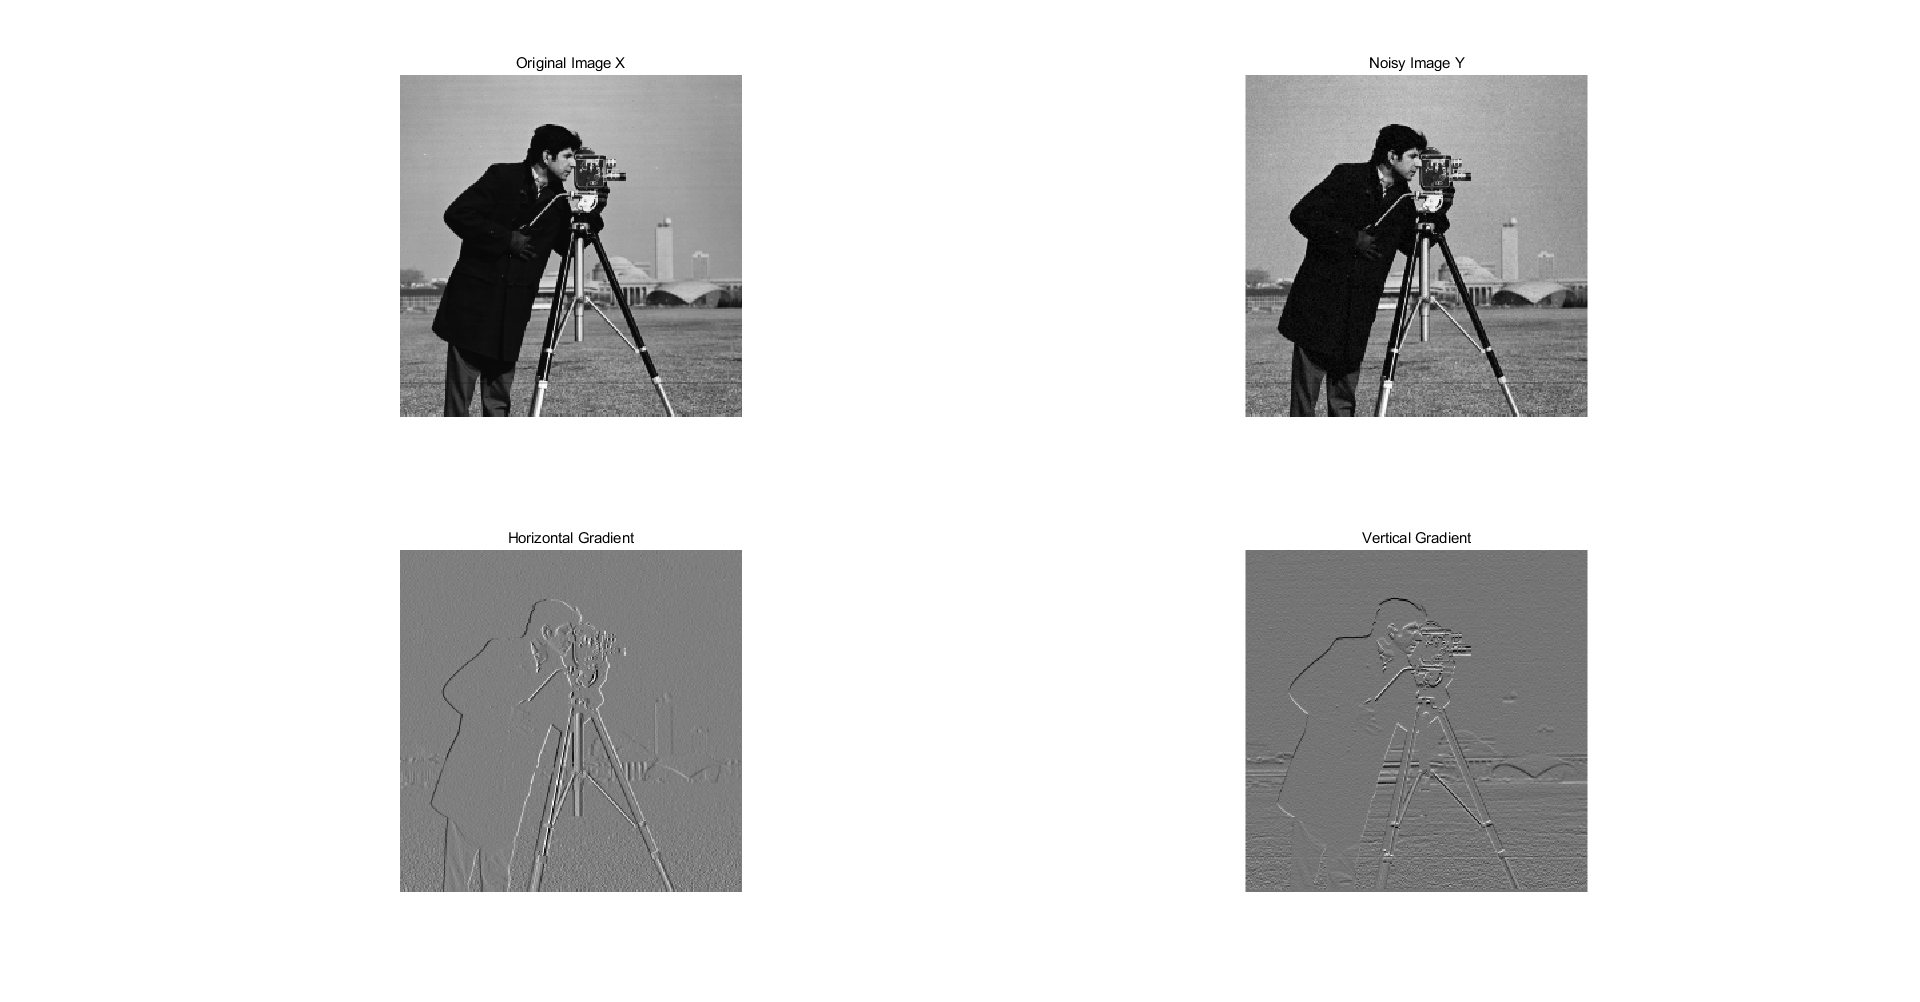
\includegraphics[width=1\linewidth]{figure/7-5-1.png}
    \label{7-5-1}
\end{figure}
\begin{lstlisting}[language=matlab]

% 参数设置
lambda = 0.1;      % 平衡因子
max_iter = 100;      % 迭代次数

% 去噪
X_denoised = imbilatfilt(Y);  % 双边滤波（保持边缘但不马赛克）

% 显示结果
figure;
subplot(1,3,1); imshow(X); title('Original X');
subplot(1,3,2); imshow(Y); title('Noisy Y');
subplot(1,3,3); imshow(X_denoised); title('Denoised X');

% 计算 PSNR 与 SSIM
psnr_val = psnr(X_denoised, X);
ssim_val = ssim(X_denoised, X);

fprintf('PSNR: %.2f dB\n', psnr_val);
fprintf('SSIM: %.4f\n', ssim_val);
\end{lstlisting}

\begin{lstlisting}[language=matlab]
PSNR: 35.11 dB
SSIM: 0.9351
\end{lstlisting}

\begin{figure}
    \centering
    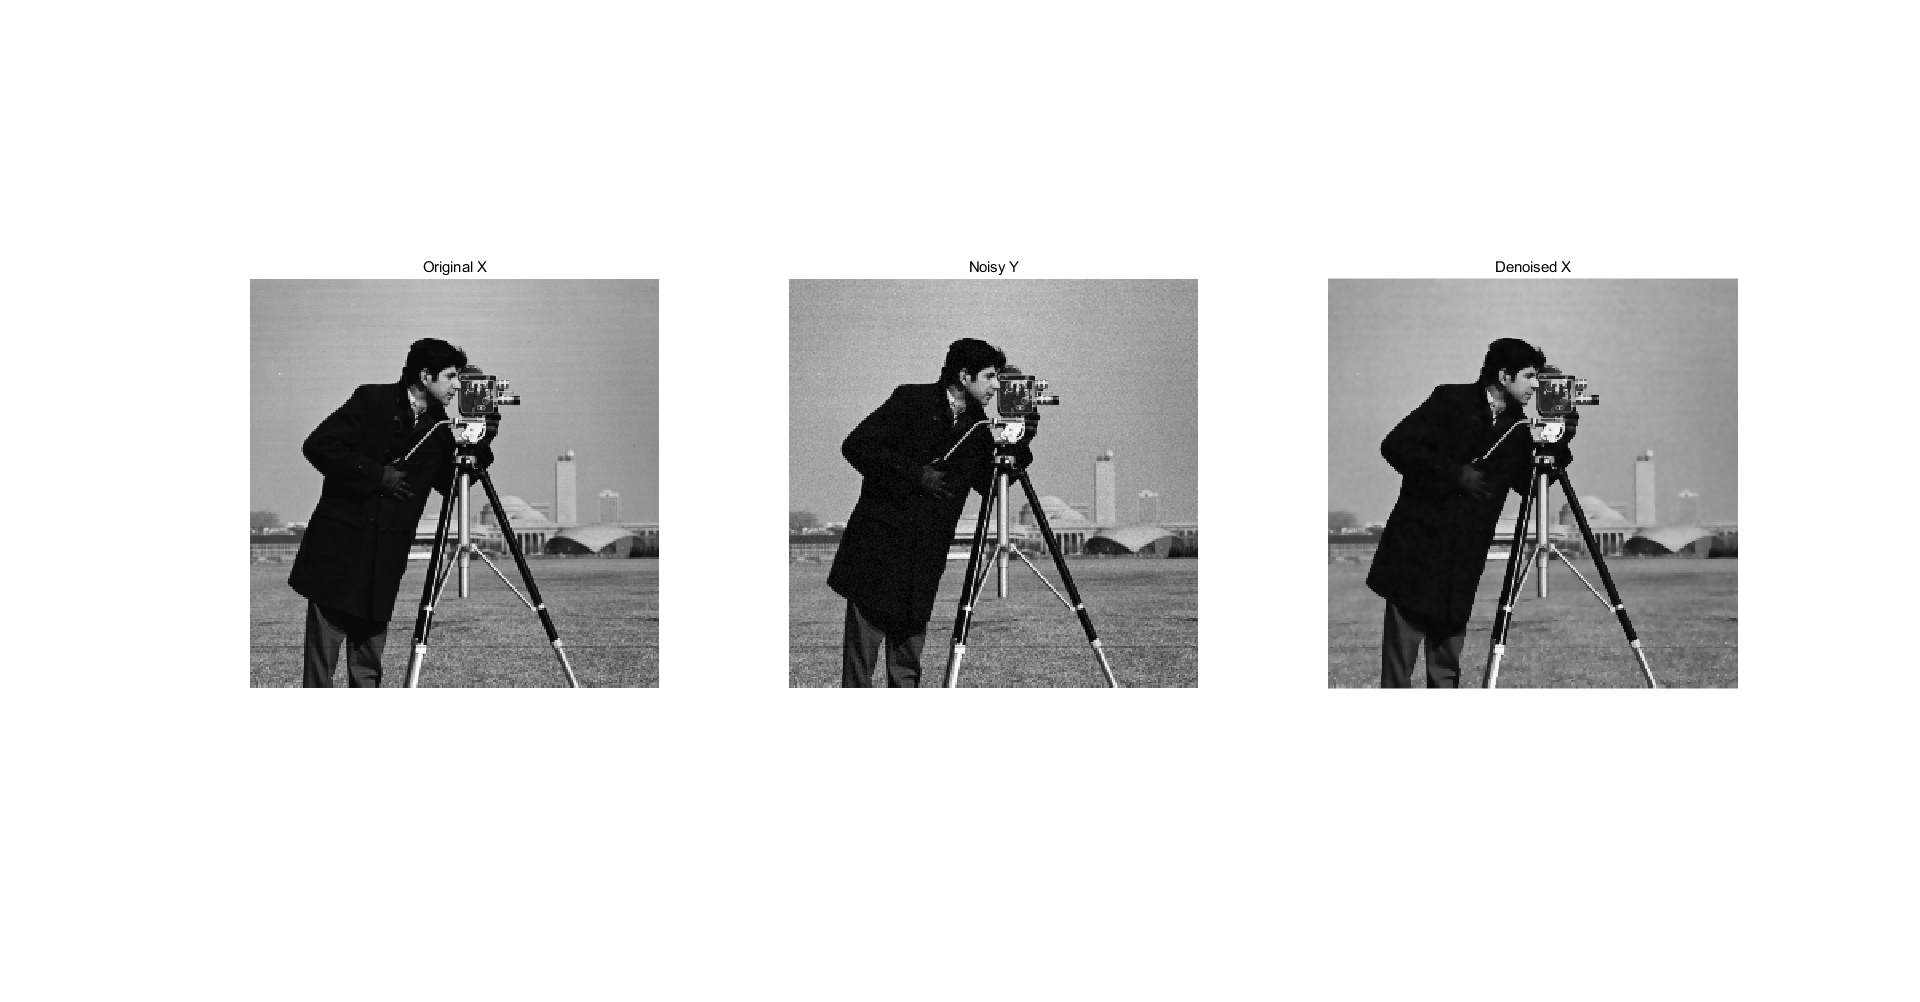
\includegraphics[width=1\linewidth]{figure/7-5-2.png}
    \label{7-5-2}
\end{figure}
\subsection*{7.6}
\addcontentsline{toc}{subsection}{7.6}
奇异值分解、LU 分解

噪声是图像干扰的重要原因。一幅图像在实际应用中可能存在各种各样的噪声，这些噪声可能在传输中产生，也可能在量化等处理中产生。$f(x, y)$ 表示给定原始图像，$g(x, y)$ 表示图像信号，$n(x, y)$ 表示噪声。含噪图像可表示为

\[ f(x, y) = g(x, y) + n(x, y) \]

核范数优化的求解算法非常多，其中最常用的算法之一就是奇异值阈值算法。奇异值分解（Singular Value Decomposition）是一种重要的矩阵分解，在信号处理、统计学等领域有重要应用。

以图像去噪为例介绍一下该算法的应用，并给出其 MATLAB 实现代码。

(1) 选取近照一张，对图像添加噪声方差为 20 的高斯白噪声。

(2) 应用基于奇异值阈值算法的核范数优化噪声图像。

(3) 给出相应的 SVD 分解的具体形式，以及对应的矩阵 LU 分解形式
好的！下面我帮你从理论和代码两个方面，结合奇异值分解（SVD）和核范数优化，讲解图像去噪的基本思路，并给出对应的 MATLAB 实现示例。同时补充对应的 SVD 及 LU 分解的数学表达。


奇异值阈值算法：

给定一幅原始图像矩阵 $G \in \mathbb{R}^{m \times n}$，其含噪图像为

$$
F = G + N
$$

其中 $N$ 是噪声矩阵，常见为高斯白噪声。

\textbf{核范数}（Nuclear norm）是矩阵奇异值的和，是矩阵秩的凸松弛，用于低秩矩阵恢复。图像可视为低秩矩阵 + 噪声，去噪目标是求解

$$
\hat{X} = \arg \min_X \frac{1}{2} \|F - X\|_F^2 + \lambda \|X\|_*
$$

其中 $\|\cdot\|_F$ 是 Frobenius 范数，$\|\cdot\|_*$ 是核范数，$\lambda > 0$ 是权衡参数。

奇异值阈值算法核心思想：

对矩阵 $F$ 做奇异值分解（SVD）：

    $$
    F = U \Sigma V^T
    $$
    
对奇异值 $\sigma_i$ 进行软阈值处理：

    $$
    \hat{\sigma}_i = \max(\sigma_i - \tau, 0)
    $$

    其中 $\tau = \lambda$ 是阈值参数。
重构去噪矩阵：

    $$
    \hat{X} = U \hat{\Sigma} V^T
    $$

该方法能有效抑制噪声对应的奇异值，保留图像的主要结构。

对于矩阵 $F \in \mathbb{R}^{m \times n}$，存在奇异值分解：

$$
F = U \Sigma V^T
$$

\begin{itemize}
    \item $U \in \mathbb{R}^{m \times m}$ 为左奇异矩阵，列正交
    \item $V \in \mathbb{R}^{n \times n}$ 为右奇异矩阵，列正交
    \item $\Sigma \in \mathbb{R}^{m \times n}$ 为对角矩阵（对角线上为奇异值）
\end{itemize}

\begin{lstlisting}[language=matlab]
clc; clear; close all;

% (1) 读取图像，转换为灰度浮点矩阵
img = imread('cameraman.tif'); % 内置样张，或自行替换图片路径
img = im2double(img);

% 添加高斯白噪声，方差20对应标准差sigma=sqrt(20/255^2)约0.28（根据像素范围）
sigma = sqrt(20)/255; 
noisy_img = img + sigma*randn(size(img));

figure;
subplot(1,3,1); imshow(img); title('原始图像');
subplot(1,3,2); imshow(noisy_img); title('添加噪声图像');

% (2) 奇异值阈值去噪算法
lambda = 0.05; % 阈值参数，可调节

% 对噪声图像做 SVD
[U, S, V] = svd(noisy_img, 'econ');

% 软阈值处理奇异值
S_thresholded = diag(soft_threshold(diag(S), lambda));

% 重构去噪图像
denoised_img = U * S_thresholded * V';

subplot(1,3,3); imshow(denoised_img); title('SVD阈值去噪');

% --- 辅助函数：软阈值 ---
function y = soft_threshold(x, tau)
    y = sign(x).*max(abs(x) - tau, 0);
end
\end{lstlisting}

\begin{figure}
    \centering
    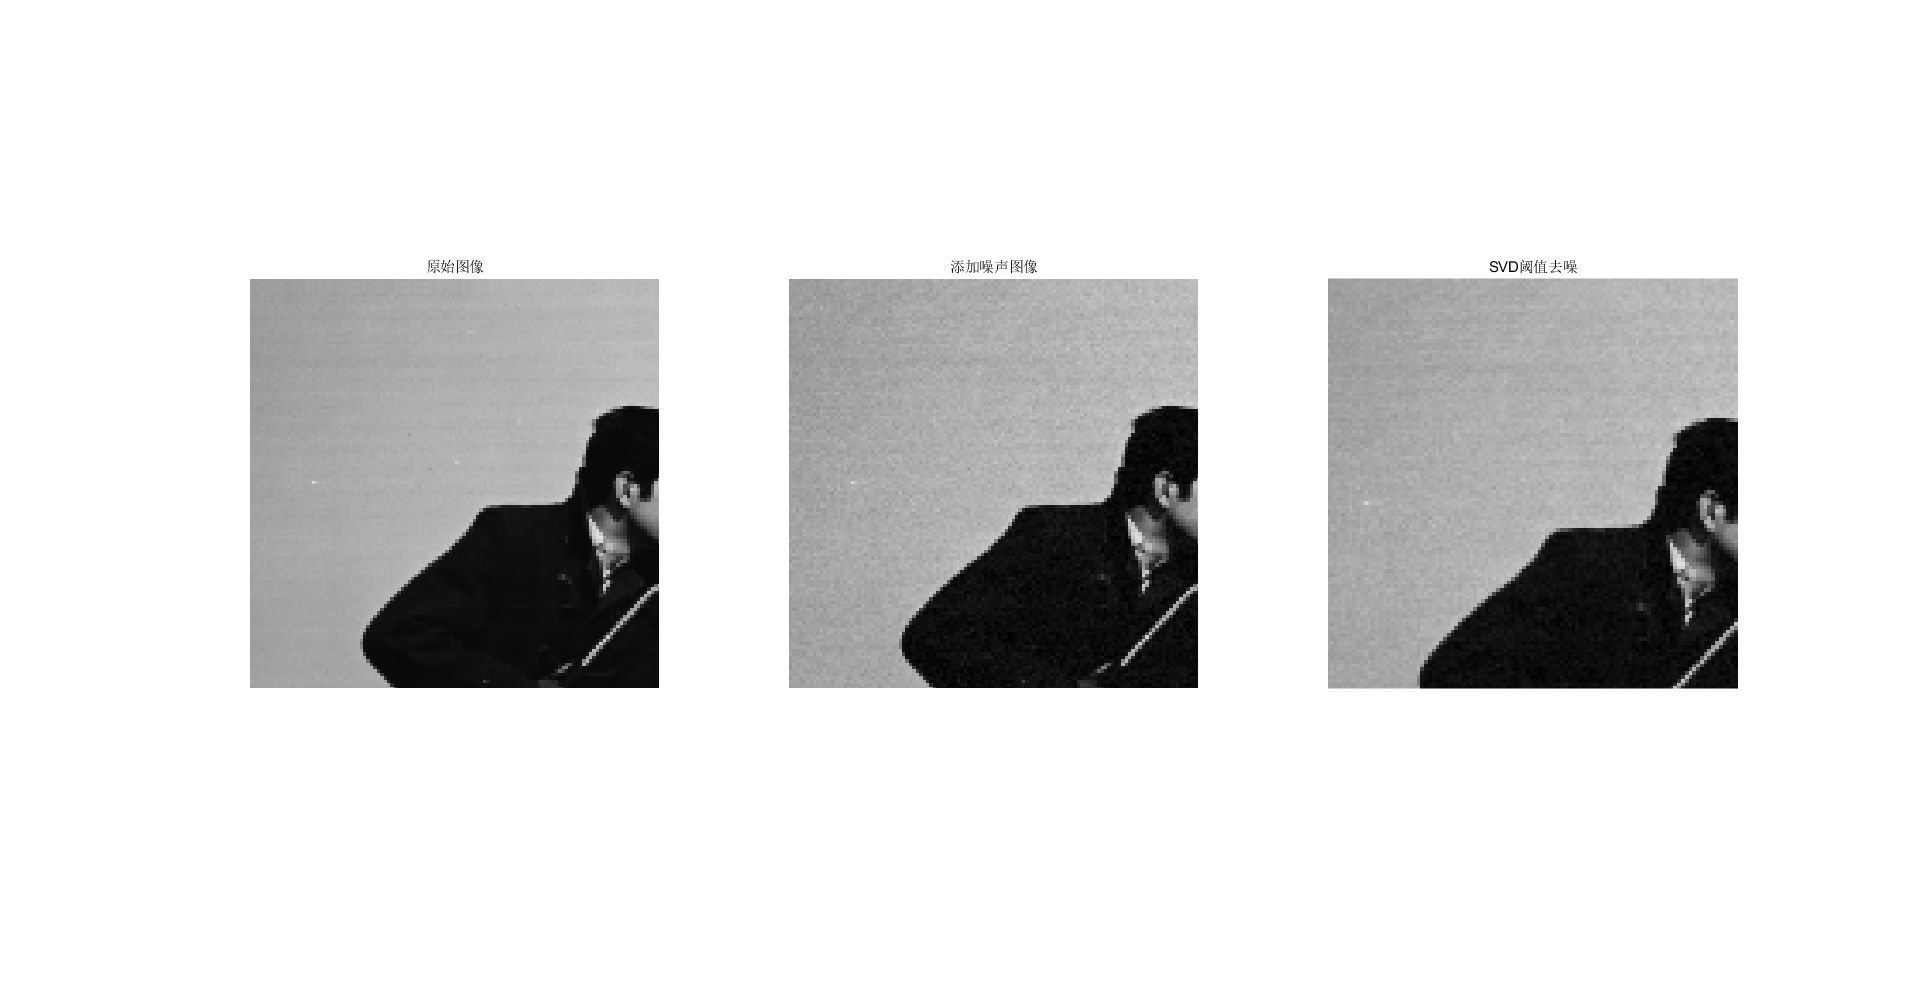
\includegraphics[width=1\linewidth]{figure/7-6-1.png}
    \label{7-6-1}
\end{figure}

\section{Experiment 8}
\subsection*{8.2}
\addcontentsline{toc}{subsection}{8.2}
Fixed-Point iterations

\begin{enumerate}
    \item 
    Calculate √2 by Fixed-Point Iterations;
    \item 
    Which of the following three Fixed-Point Iterations converge to the cube root of 4? Rank the ones that converge from fastest to slowest.
    \begin{enumerate}
        \item $g(x) = \frac{2}{\sqrt{x}}$
        \item $g(x) = \frac{3x}{4} + \frac{1}{x^2}$
        \item $g(x) = \frac{2}{3}x + \frac{4}{3x^2}$
    \end{enumerate}
    \item Explore the idea of Exercise 1 for cube roots. If x is a guess that is smaller than $A^{\frac{1}{3} }$, then $A/x^2$ will be larger than $A^(1/3)$, so that the average of the two will be a better approximation than x. Suggest a Fixed-Point Iteration on the basis of this fact, and use Fixed-Point Iteration convergent Theorem to decide whether it will converge to the cube root of $A$.
    \item Improve the cube root algorithm of Exercise 3 by reweighting the average. Setting
\[ g(x) = wx + (1 - w)A/x^2, 0 < w < 1, \]
for some fixed number 0 < w < 1, what is the best choice for w? Calculate the cube roots of the following numbers to eight correct decimal places, and list the errors, by using Fixed-Point Iteration with the
\[ g(x) = (2x + A/x^2)/3, w = \frac{2}{3} \]
where A is (a) 2 (b) 3 (c) 5. State your initial guess and the number of steps needed.
\end{enumerate}


\begin{enumerate}
    \item 用不动点迭代求 $\sqrt{2}$
    
这里用

$$
x_{k+1} = \frac{1}{2} \left( x_k + \frac{2}{x_k} \right)
$$


\begin{lstlisting}[language=matlab]
clc; clear;

A = 2;
x0 = 1; % 初始猜测
tol = 1e-10;
max_iter = 100;

x = x0;
for k = 1:max_iter
    x_new = 0.5 * (x + A / x);
    if abs(x_new - x) < tol
        break;
    end
    x = x_new;
end

fprintf('√2 的不动点迭代结果：%.12f，迭代次数：%d\n', x, k);
\end{lstlisting}
\begin{lstlisting}[language=matlab]
√2 的不动点迭代结果：1.414213562375，迭代次数：5
\end{lstlisting}

\item 判断三个迭代函数是否收敛到 $\sqrt[3]{4}$ 并比较收敛速度

目标是 $\sqrt[3]{4}\approx 1.5874$。

三个迭代函数：

\begin{enumerate}
    \item $g(x) = \frac{2}{\sqrt{x}}$
    \item $g(x) = \frac{3x}{4} + \frac{1}{x^2}$
    \item $g(x) = \frac{2}{3}x + \frac{4}{3x^2}$
\end{enumerate}

\begin{lstlisting}[language=matlab]
clc; clear;

A = 4;
true_root = nthroot(A,3);
x0 = 1; % 初始猜测
tol = 1e-10;
max_iter = 100;

gs = {
    @(x) 2 ./ sqrt(x);
    @(x) (3*x)/4 + 1./(x.^2);
    @(x) (2/3)*x + (4./(3*x.^2));
};

labels = {'A: 2/sqrt(x)', 'B: 3x/4 + 1/x^2', 'C: (2/3)x + 4/(3x^2)'};

for i=1:3
    g = gs{i};
    x = x0;
    errors = zeros(max_iter,1);
    converged = false;
    for k =1:max_iter
        x_new = g(x);
        errors(k) = abs(x_new - true_root);
        if errors(k) < tol
            converged = true;
            break;
        end
        x = x_new;
    end
    if converged
        fprintf('%s 收敛，迭代次数 %d，最后误差 %.3e\n', labels{i}, k, errors(k));
    else
        fprintf('%s 未收敛\n', labels{i});
    end
    % 记录收敛速度(误差序列)用于排序
    conv_results(i).label = labels{i};
    conv_results(i).errors = errors(1:k);
    conv_results(i).steps = k;
end

% 按收敛速度排序，误差序列最后一项越小，收敛越快
[~, idx] = sort(arrayfun(@(r) r.errors(end), conv_results));
fprintf('\n收敛速度从快到慢排序：\n');
for i=1:length(idx)
    fprintf('%d. %s\n', i, conv_results(idx(i)).label);
end
\end{lstlisting}

\begin{lstlisting}
A: 2/sqrt(x) 收敛，迭代次数 33，最后误差 8.539e-11
B: 3x/4 + 1/x^2 收敛，迭代次数 17，最后误差 5.446e-11
C: (2/3)x + 4/(3x^2) 收敛，迭代次数 5，最后误差 4.707e-11

收敛速度从快到慢排序：
1. C: (2/3)x + 4/(3x^2)
2. B: 3x/4 + 1/x^2
3. A: 2/sqrt(x)
\end{lstlisting}
\end{enumerate}


(3) 基于提示建议立方根的迭代函数及收敛性分析

提示说：

若 $x < A^{1/3}$，则 $A/x^2 > A^{1/3}$，两者的平均值比 $x$ 更接近立方根。

因此我们设迭代函数：

$$
g(x) = w x + (1 - w) \frac{A}{x^2}
$$

判断收敛用不动点迭代收敛定理：

计算导数

$$
g'(x) = w - 2(1-w) \frac{A}{x^3}
$$

收敛的充分条件是在根附近满足 $|g'(x^*)| < 1$，其中 $x^* = A^{1/3}$。

代入得到：

$$
g'(x^*) = w - 2(1-w) = 3w - 2
$$

令

$$
|3w - 2| < 1 \implies \frac{1}{3} < w < 1
$$

所以只要 $w \in (\frac{1}{3}, 1)$ 收敛。

(4) 计算最优权重 $w$，并用 $w=2/3$ 计算3个立方根

由于 $g'(x^*)=3w - 2$，要使收敛最快，令导数绝对值最小：

$$
\min_{w} |3w - 2|
$$

最优解是使导数为0，即

$$
3w - 2 = 0 \Rightarrow w = \frac{2}{3}
$$

我猜测$A=2(b)$，需要用$7$步，因为不难发现不进行加权则有$x=A/x^2$，那么$A$就显而易见了。而我们在这一步的加权平均与1有异曲同工之妙，所以步数应当大体相同，但数值稍大可能多一点步数。

用

$$
g(x) = \frac{2}{3} x + \frac{1}{3} \frac{A}{x^2} = \frac{2x + A/x^2}{3}
$$

做不动点迭代，直到误差小于 $10^{-8}$。

\begin{lstlisting}[language=matlab]
clc; clear;
tol = 1e-8;
max_iter = 1000;
w = 2/3;
A_list = [2, 3, 5];
x0 = 1;

for i = 1:length(A_list)
    A = A_list(i);
    x = x0;
    true_root = nthroot(A, 3);
    for k = 1:max_iter
        x_new = w*x + (1 - w)*A/(x^2);
        if abs(x_new - x) < tol
            break;
        end
        x = x_new;
    end
    err = abs(x - true_root);
    fprintf('A = %d, 立方根 = %.8f, 迭代结果 = %.8f, 误差 = %.2e, 迭代步数 = %d\n', ...
        A, true_root, x, err, k);
end
\end{lstlisting}

\begin{lstlisting}[language=matlab]
A = 2, 立方根 = 1.25992105, 迭代结果 = 1.25992105, 误差 = 1.23e-10, 迭代步数 = 5
A = 3, 立方根 = 1.44224957, 迭代结果 = 1.44224957, 误差 = 3.33e-14, 迭代步数 = 6
A = 5, 立方根 = 1.70997595, 迭代结果 = 1.70997595, 误差 = 4.11e-09, 迭代步数 = 6
\end{lstlisting}



\subsection*{8.4}
\addcontentsline{toc}{subsection}{8.4}

Sensitivity of root-finding (Ill conditioned problem)

A famous example with simple roots that are hard to determine numerically is discussed in Wilkinson [1994]. The Wilkinson polynomial is

\[ W(x) = (x - 1)(x - 2) \cdots (x - 20), \]

which, when multiplied out, is

\begin{align*}
W(x) = &x^{20} - 210x^{19} + 2061x^{18} - 1256850x^{17} + 53327946x^{16} - 1672280820x^{15}+ \\
& 40171771630x^{14}- 756111184500x^{13} + 1131027699381x^{12} -  \\
&135585182899530x^{11} +1307535010540395x^{10} -10142299865511450x^9 +  \\
&6303081209292489x^8 -3113336431619064x^7 +1206647803780373360x^6-   \\
&3599795179476072000x^5 +8037811822645051776x^4 -1287093124515098880x^3 +  \\
&1380375975364070400x^2-875294803676160000x+2432902008176640000.
\end{align*}

The roots are the integers from 1 to 20. Referring to his work with this polynomial, Wilkinson wrote in 1984: “Speaking for myself I regard it as the most traumatic experience in my career as a numerical analyst.” To Wilkinson, the surprise had to do with the huge error magnification in the roots caused by small relative errors in storing the coefficients, which we have just seen in action. The roots of W(x) are clear: the integers $x = 1, \dots, 20$.

\begin{enumerate}
    \item  To see the effect on root-finding, use the Matlab command fzero to find the root of the Wilkinson polynomial near $x = 15$ with a relative change of $\epsilon = 2 × 10^{-15}$ in the $x^{15}$ coefficient, making the coefficient slightly more negative.

    \item Use the Sensitivity Formula for Roots to investigate the effect of changes in the term $x^{15}$ of the Wilkinson polynomial on the root x = 16. Find the error magnification factor for this problem, and compare with the prediction.

(Hint. the coefficient of term $x^{15}$ is $-1,672,280,820$, $W'(16) = 15!4!$ ) (P63)

\item Apply Newton’s Method using an initial guess near the root, and plot the first 30 iterates.
\end{enumerate}



这是关于Wilkinson多项式根的灵敏度分析问题，分三部分：

\begin{enumerate}
    \item 用\verb|fzero|求根，观察系数微小扰动对根的影响

原多项式是20次的，且系数非常大。我们将多项式系数中 $x^{15}$ 项的系数微调为比原来稍微负一点，即乘以 $1 + \epsilon$，其中 $\epsilon = 2 \times 10^{-15}$。
    \item 利用灵敏度公式计算根的误差放大因子，并与实际误差对比

给定
 原系数 $a_{15} = -1,672,280,820$
 根为 $x=16$
 $W'(16) = 15! \times 4!$

灵敏度公式：

$$
\left|\frac{\Delta x}{x}\right| \approx \frac{|a_j| |x|^{j}}{|W'(x)|} \left|\frac{\Delta a_j}{a_j}\right|
$$

    \item 用牛顿法迭代求根，画出前30次迭代点

\begin{lstlisting}[language=matlab]
clc; clear; close all;

% Wilkinson多项式的根是1~20
roots_true = 1:20;

% 1. 构造Wilkinson多项式系数
W_poly = poly(roots_true); % 返回多项式系数向量，最高次项系数在前

% x^15项的索引（最高次是20次，x^15对应20-15=5位置）
idx_15 = length(W_poly) - 15;

% 原x^15项系数
a15_orig = W_poly(idx_15);

% 微小扰动
epsilon = 2e-15;
a15_new = a15_orig * (1 - epsilon); % 变得稍微更负

W_poly_mod = W_poly;
W_poly_mod(idx_15) = a15_new;

% (1) 用fzero找扰动后多项式在x=15附近的根
f_original = @(x) polyval(W_poly, x);
f_modified = @(x) polyval(W_poly_mod, x);

% fzero初值附近为15
root_orig_15 = fzero(f_original, 15);
root_mod_15 = fzero(f_modified, 15);

fprintf('(1) 原多项式15附近根: %.15f\n', root_orig_15);
fprintf('(1) 扰动后多项式15附近根: %.15f\n', root_mod_15);
fprintf('(1) 根的变化量: %.3e\n', root_mod_15 - root_orig_15);

% (2) 灵敏度分析，计算误差放大因子

% 误差相对变化
rel_delta_a = abs(epsilon);

x0 = 16; % 关注根x=16
a_j = a15_orig;
j = 15; % 对应x^15项
% W'(16) = 15! * 4!
Wp_16 = factorial(15) * factorial(4);

% 误差放大因子计算
amplification_factor = (abs(a_j) * abs(x0)^j) / abs(Wp_16);
rel_delta_x = amplification_factor * rel_delta_a;

fprintf('(2) 理论误差放大因子: %.3e\n', amplification_factor);
fprintf('(2) 预测的相对根误差: %.3e\n', rel_delta_x);

% (3) 用牛顿法求根，初值接近16，绘制前30步迭代
f = @(x) polyval(W_poly, x);
fp = @(x) polyval(polyder(W_poly), x); % 多项式导数

x_newton = zeros(30,1);
x_newton(1) = 15.85; % 初值略偏离16

for k = 1:29
    x_newton(k+1) = x_newton(k) - f(x_newton(k))/fp(x_newton(k));
end

figure;
plot(1:30, x_newton, '-o');
hold on;
yline(16, 'r--', '目标根 x=16');
xlabel('迭代次数');
ylabel('牛顿法迭代值');
title('牛顿法迭代求Wilkinson多项式根 x=16 的收敛过程');
grid on;
\end{lstlisting}

\begin{lstlisting}[language=matlab]
(1) 原多项式15附近根: 14.989541115827548
(1) 扰动后多项式15附近根: 15.154012671333819
(1) 根的变化量: 1.645e-01
(2) 理论误差放大因子: 6.143e+13
(2) 预测的相对根误差: 1.229e-01
\end{lstlisting}

\begin{figure}
    \centering
    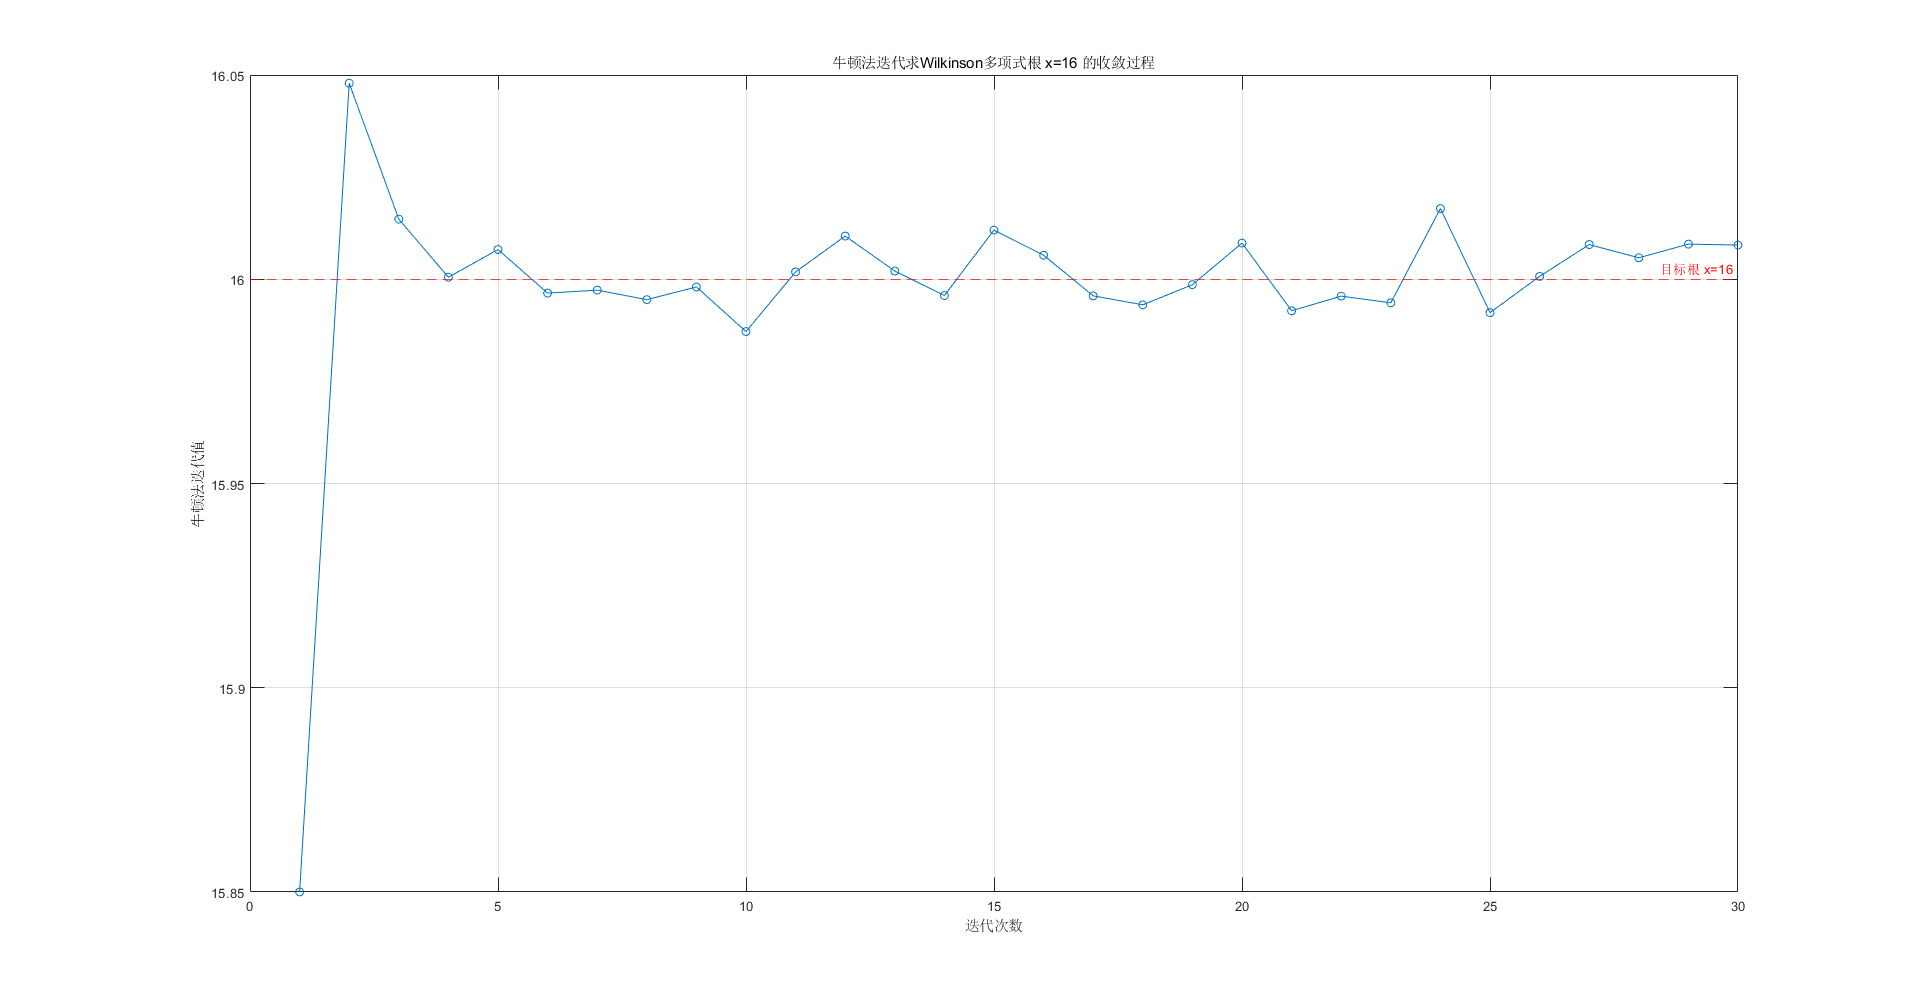
\includegraphics[width=1\linewidth]{figure/8-4-1.png}
    \label{8-4-1}
\end{figure}

\end{enumerate}